%===============================================================================
% LaTeX sjabloon voor de bachelorproef toegepaste informatica aan HOGENT
% Meer info op https://github.com/HoGentTIN/bachproef-latex-sjabloon
%===============================================================================

\documentclass{bachproef-tin}

\usepackage{hogent-thesis-titlepage} % Titelpagina conform aan HOGENT huisstijl
\usepackage{lipsum}
\usepackage{biblatex}

\bibliography{bachproef-tin.bib}{}

%%---------- Documenteigenschappen ---------------------------------------------
% TODO: Vul dit aan met je eigen info:

% De titel van het rapport/bachelorproef
\title{Microservice integration patterns op SAP order-to-cash proces.}

% Je eigen naam
\author{Lyva Van Damme}

% De naam van je promotor (lector van de opleiding)
\promotor{Karine Samyn}

% De naam van je co-promotor. Als je promotor ook je opdrachtgever is en je
% dus ook inhoudelijk begeleidt (en enkel dan!), mag je dit leeg laten.
\copromotor{Nicolas Pauwelyn}

% Indien je bachelorproef in opdracht van/in samenwerking met een bedrijf of
% externe organisatie geschreven is, geef je hier de naam. Zoniet laat je dit
% zoals het is.
\instelling{HoGent}

% Academiejaar
\academiejaar{2018-2019}

% Examenperiode
%  - 1e semester = 1e examenperiode => 1
%  - 2e semester = 2e examenperiode => 2
%  - tweede zit  = 3e examenperiode => 3
\examenperiode{3}

%===============================================================================
% Inhoud document
%===============================================================================

\begin{document}

%---------- Taalselectie -------------------------------------------------------
% Als je je bachelorproef in het Engels schrijft, haal dan onderstaande regel
% uit commentaar. Let op: de tekst op de voorkaft blijft in het Nederlands, en
% dat is ook de bedoeling!

%\selectlanguage{english}

%---------- Titelblad ----------------------------------------------------------
\inserttitlepage

%---------- Samenvatting, voorwoord --------------------------------------------
\usechapterimagefalse
%%=============================================================================
%% Voorwoord
%%=============================================================================

\chapter*{\IfLanguageName{dutch}{Woord vooraf}{Preface}}
\label{ch:voorwoord}

%% TODO:
%% Het voorwoord is het enige deel van de bachelorproef waar je vanuit je
%% eigen standpunt (``ik-vorm'') mag schrijven. Je kan hier bv. motiveren
%% waarom jij het onderwerp wil bespreken.
%% Vergeet ook niet te bedanken wie je geholpen/gesteund/... heeft
Deze bachelorproef werd geschreven om het behalen van het bachelordiploma Toegepaste Informatica. Eerst was het niet gemakkelijk om een onderwerp te vinden. Ik zou daarom graag mijn stagebedrijf, delaware, willen bedanken voor het voorstellen van het onderwerp: Microservice integration patterns op SAP order-to-cash proces. Dankzij hen kon ik mijn bachelorproef doen over een onderwerp dat mij echt interesseerde. Het was een aangename ervaring om drie jaar van de opleiding te kunnen omzetten in dit eindwerk. De ervaring van andere mensen heeft mij geholpen om door deze periode te geraken.
Als eerste wil ik mijn co-promotor, Nicolas Pauwelyn, bedanken voor zijn hulp.
Ik zou graag mijn ouders bedanken voor de steun en hun geduld tijdens de stressvolle situaties. Ook wil ik mijn broer en zus bedanken voor hun steun.
Als laatste zou ik graag mijn medestudenten bedanken voor alle hulp die ze mij gaven. 

%%=============================================================================
%% Samenvatting
%%=============================================================================

% TODO: De "abstract" of samenvatting is een kernachtige (~ 1 blz. voor een
% thesis) synthese van het document.
%
% Deze aspecten moeten zeker aan bod komen:
% - Context: waarom is dit werk belangrijk?
% - Nood: waarom moest dit onderzocht worden?
% - Taak: wat heb je precies gedaan?
% - Object: wat staat in dit document geschreven?
% - Resultaat: wat was het resultaat?
% - Conclusie: wat is/zijn de belangrijkste conclusie(s)?
% - Perspectief: blijven er nog vragen open die in de toekomst nog kunnen
%    onderzocht worden? Wat is een mogelijk vervolg voor jouw onderzoek?
%
% LET OP! Een samenvatting is GEEN voorwoord!

%%---------- Nederlandse samenvatting -----------------------------------------
%
% TODO: Als je je bachelorproef in het Engels schrijft, moet je eerst een
% Nederlandse samenvatting invoegen. Haal daarvoor onderstaande code uit
% commentaar.
% Wie zijn bachelorproef in het Nederlands schrijft, kan dit negeren, de inhoud
% wordt niet in het document ingevoegd.

\IfLanguageName{english}{%
\selectlanguage{dutch}
\chapter*{Samenvatting}

\selectlanguage{english}
}{}

%%---------- Samenvatting -----------------------------------------------------
% De samenvatting in de hoofdtaal van het document

\chapter*{\IfLanguageName{dutch}{Samenvatting}{Abstract}}

% CONTEXT

% NOOD
'Microservice integration patterns op SAP order-to-cash proces' werd voorgesteld door delaware om te onderzoeken hoe microservice integration patterns een invloed kunnen hebben op het order-to-cash proces binnen SAP. 

% TAAK
Dit onderzoek kent een verdiepende structuur. Als eerst zal er uitleg worden gegeven omtrent microservices, dan komt er een vergelijking tussen de verschillende onderdelen. Enkele voorbeelden hiervan zijn authenticatie en authorisatie. Deze scriptie sluit af met opkomende ideologieën en de bescherming van microservices.

% OBJECT
In deze thesis is als eerste een uitgebreide literatuurstudie terug te vinden. In deze studie wordt er dieper ingegaan op de technologie van microservices en de verschillende integration patterns daaromtrent. Daarnaast zal er meer uitleg gegeven worden over het order-to-cash proces.
Na de literatuurstudie wordt een microservice integration pattern toegepast op het order-to-cash proces. Als afsluiter komt de conclusie omtrent deze studie.

% RESULTAAT
Microservices zorgen voor een geautomatiseerd proces met weinig menselijke interactie, het is een complexe architectuur. De overschakeling naar een microservice architectuur bevat veel onderdelen waar er in eerste instantie niet aan gedacht wordt. Het werd ook duidelijk dat er goed moet worden nagedacht over alle kleine dingen, zoals authenticatie, de manier van bescherming, hoe logging wordt opgevangen...
De manier op microservices te gaan gebruiken binnen een architectuur kan aan de hand van integration patterns. Er kan een microservice architectuur opgezet worden aan de hand van één integration pattern maar dat is niet aangeraden. Elke integration pattern heeft zijn tekortkomingen. Door meerdere te gaan combineren is de kans op falen kleiner, mits deze goed worden toegepast.

% CONCLUSIE
De overschakeling kan gemakkelijk onderschat worden waardoor zich een belangrijke vraag is: hebben microservices wel een meerwaarde in dit proces? Of de overschakeling moet gemaakt worden, is afhankelijk van wat de noden van de applicatie precies zijn.

% PERSPECTIEF
Er zullen zeker vragen en aanvullingen komen in de toekomst. Dit is een evoluerende technologie en er zullen betere oplossingen komen voor de verschillende onderdelen.

%---------- Inhoudstafel -------------------------------------------------------
\pagestyle{empty} % Geen hoofding
\tableofcontents  % Voeg de inhoudstafel toe
\cleardoublepage  % Zorg dat volgende hoofstuk op een oneven pagina begint
\pagestyle{fancy} % Zet hoofding opnieuw aan

%---------- Lijst figuren, afkortingen, ... ------------------------------------

% Indien gewenst kan je hier een lijst van figuren/tabellen opgeven. Geef in
% dat geval je figuren/tabellen altijd een korte beschrijving:
%
%  \caption[korte beschrijving]{uitgebreide beschrijving}
%
% De korte beschrijving wordt gebruikt voor deze lijst, de uitgebreide staat bij
% de figuur of tabel zelf.

\listoffigures
\listoftables

% Als je een lijst van afkortingen of termen wil toevoegen, dan hoort die
% hier thuis. Gebruik bijvoorbeeld de ``glossaries'' package.
% https://www.overleaf.com/learn/latex/Glossaries

%---------- Kern ---------------------------------------------------------------

% De eerste hoofdstukken van een bachelorproef zijn meestal een inleiding op
% het onderwerp, literatuurstudie en verantwoording methodologie.
% Aarzel niet om een meer beschrijvende titel aan deze hoofstukken te geven of
% om bijvoorbeeld de inleiding en/of stand van zaken over meerdere hoofdstukken
% te verspreiden!

%%=============================================================================
%% Inleiding
%%=============================================================================

\chapter{\IfLanguageName{dutch}{Inleiding}{Introduction}}
\label{ch:inleiding}

\section{\IfLanguageName{dutch}{Probleemstelling}{Problem Statement}}
\label{sec:probleemstelling}
De promotor en doelgroep van dit onderzoek is delaware. Zij stelden voor om te onderzoeken hoe microservices integration patterns het order-to-cash proces beïnvloeden. Microservices is een opkomende technologie die invloed heeft op de architectuur van een applicatie. Omtrent deze technologie zijn er verschillende manieren, integration patterns, om te implementeren. Het nut van deze bachelorproef is om integration patterns op een order-to-cash proces toe te passen, op een theoretisch vlak. Op die manier kan er een beeld geschetst worden om bij een bestaande architectuur deze nieuwe technologie te gebruiken.

\section{\IfLanguageName{dutch}{Onderzoeksvraag}{Research question}}
\label{sec:onderzoeksvraag}
De onderzoeksvraag is: "Hoe microservice integration patterns een order-to-cash proces in SAP kan beïnvloeden?". Of de beïnvloeding positief of negatief is, zal later duidelijk worden. De algemene vraag delen we op in volgende punten:
\begin{itemize}
  \item Wat zijn microservices?
  \item Welke aanpassingen kunnen of moeten er gebeuren aan de architectuur om de microservices te laten werken?
  \item Hoe zal de communicatie tussen de verschillende microservices werken?
  \item Welke integration patterns zijn er?
  \item Hoe ziet een order-to-cash (OTC) proces er uit?
  \item Welke business requirements heeft een order-to-cash proces?
  \item Welke invloed heeft een microservice integration pattern op het order-to-cash proces?
\end{itemize}
Dit zal een theoretische studie zijn.

\section{\IfLanguageName{dutch}{Onderzoeksdoelstelling}{Research objective}}
\label{sec:onderzoeksdoelstelling}
Het doel van deze paper is het onderzoeken van de effecten van een microservices integration patterns op de architectuur van een OTC-proces in SAP. De ambitie houdt in dat er verschillende microservice integration patterns worden onderzocht. Bij de methodologie wordt er één integration pattern theoretisch benaderd op het order-to-cash proces. Het integration pattern zal gekozen worden aan de hand van een vergelijking met verschillende patterns.

\section{\IfLanguageName{dutch}{Opzet van deze bachelorproef}{Structure of this bachelor thesis}}
\label{sec:opzet-bachelorproef}

% Het is gebruikelijk aan het einde van de inleiding een overzicht te
% geven van de opbouw van de rest van de tekst. Deze sectie bevat al een aanzet
% die je kan aanvullen/aanpassen in functie van je eigen tekst.

De rest van deze bachelorproef is als volgt opgebouwd:

In Hoofdstuk~\ref{ch:stand-van-zaken} wordt een overzicht gegeven van de stand van zaken binnen het onderzoeksdomein, op basis van een literatuurstudie. Hierin zal er meer uitleg gegeven worden over microservices, verschillende integration patterns en het order-to-cash proces binnen SAP.

In Hoofdstuk~\ref{ch:methodologie} wordt de methodologie toegelicht.  Hier zal het onderzoek worden uitgevoerd over hoe microservices integration patterns het order-to-cash proces beïnvloeden. 

% TODO: Vul hier aan voor je eigen hoofstukken, één of twee zinnen per hoofdstuk

In Hoofdstuk~\ref{ch:conclusie}, ten slotte, wordt de conclusie gegeven en een antwoord geformuleerd op de onderzoeksvragen. Daarbij wordt een aanzet gegeven voor toekomstig onderzoek binnen dit domein.

% !TeX spellcheck = de_DE
\chapter{\IfLanguageName{dutch}{Stand van zaken}{State of the art}}
\label{ch:stand-van-zaken}

% Tip: Begin elk hoofdstuk met een paragraaf inleiding die beschrijft hoe
% dit hoofdstuk past binnen het geheel van de bachelorproef. Geef in het
% bijzonder aan wat de link is met het vorige en volgende hoofdstuk.

% Pas na deze inleidende paragraaf komt de eerste sectiehoofding.

Dit hoofdstuk bevat de literatuurstudie omtrent het onderwerp. Hier worden de architectuur en de termen uitgelegd. Daarnaast zal hier een vergelijking gemaakt worden tussen onderdelen van microservices en zal er een beeld van een order-to-cash proces gemaakt worden.

\section{Microservices}
\subsection{Definitie}
Aangezien de term monolithic veelvuldig zal gebruikt worden, zal eerst de definitie gegeven worden:  'Monolithic software is designed to be self-contained; components of the program are interconnected and interdependent rather than loosely coupled as is the case with ' software programs.',  \textcite{Wigmore2016}.
Om te begrijpen waarom een overschakeling naar microservices een goed idee is, worden de moeilijkheden bij monolithic architectuur aangehaald. Bij een verandering binnen een monolithic architectuur wordt een geheel nieuwe versie uitgebracht. Dit creëert een aanzienlijke overhead. Met architectuur wordt de algemene manier van implementatie bedoeld. Bij het gebruik van het woord architectuur, wordt er niet verwezen naar de applicatie maar naar de achterliggende logica ervan.
De overschakeling naar microservice omvat onder andere:
\begin{itemize}
	\item de volledige architectuur moet opnieuw getest worden
	\item deze architectuur kan heel complex worden bij het toevoegen van functionaliteiten
	\item de complete architectuur moet opnieuw gedeployed worden bij elke update
	\item de impact van een verandering kan verkeerd ingeschat worden
	\item bij een fout in een proces, kan de volledige architectuur falen
\end{itemize}
Er zijn meerdere definities terug te vinden over microservices die hieronder uitgelegd staan. De uitleg is gebaseerd op definities van \textcite{Mauersberger2017}, \textcite{Watts2018} en \textcite{Benetis2016a}.

Er zijn verschillende elementen omtrent de uitleg over microservices. Een eerste onderdeel spitst zich toe op de  werking van een microservice. Het is een onafhankelijke, kleine, modulaire service. Modulaire services zijn services waarbij veel delen uitwisselbaar zijn met diverse services. Wordt er info gestuurd of gevraagd van service A, dan zal dit geen invloed hebben op de andere services. Een tweede eigenschap is de eenvoudig communicatie. Daar is nood aan omdat sommige services data moeten uitwisselen om hun 'job' te kunnen doen. De communicatie kan gebeuren op verschillende manieren. De manier die bekendst is, is 'Messaging via a Message Broker'. Dit wil zeggen dat microservice A een bericht plaatst op de wachtrij bij microservice B wanneer A data wil doorsturen. Dan kan microservice B aan die data wanneer hij die nodig heeft. Ze zullen soms moeten wachten maar ze zijn zo goed als onafhankelijk van elkaar. De derde eigenschap omvat dat een microservice wordt gemaakt in functie van een requirement uit de business. Elk product in de business heeft een doel dat moet voldoen aan eisen. Het unieke aan microservices is dat  men  ze gaat bekijken vanuit de eisen binnen de business. Het doel van microservices is, de problemen die te vinden zijn bij een monolithic, verhelpen. 
 
De verschillen tussen een monolithic en microservices kunnen het best afgebeeld worden in een afbeelding 2.1.

\begin{figure}[h!]
	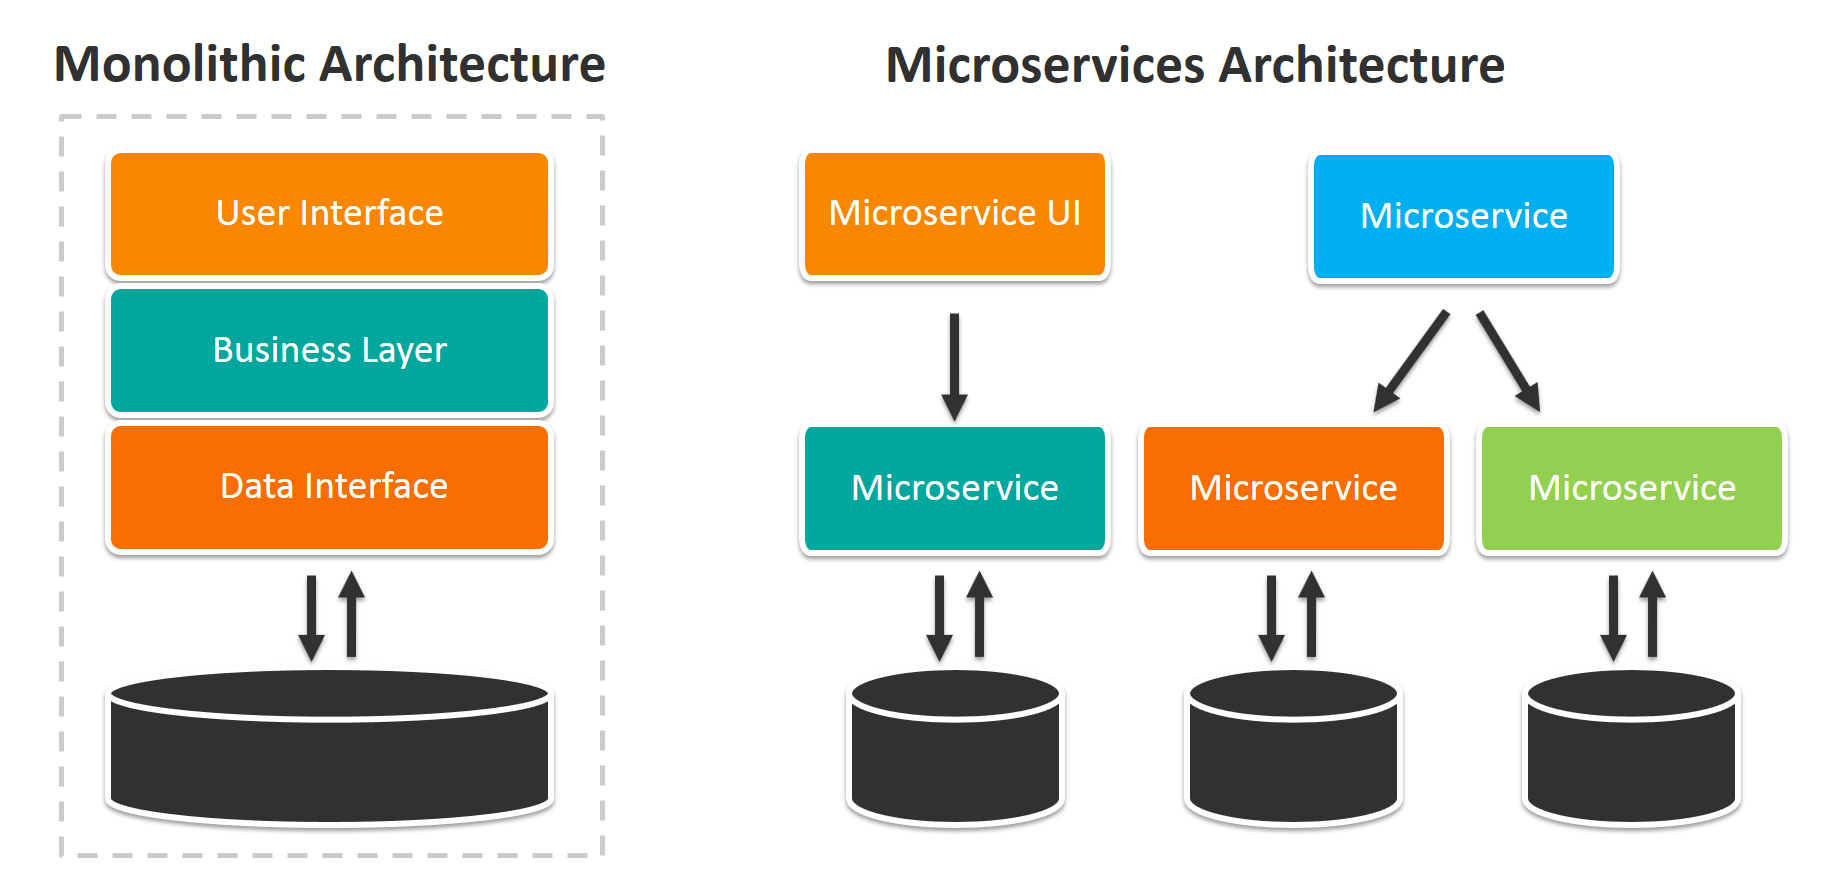
\includegraphics[width=10cm]{microservices-vs-monolithic.jpg}
	\centering
	\caption{Een monolithic architectuur naast een microservice architectuur. \textcite{Watts2018}}
\end{figure}
 De monolithic wordt  weergegeven in de linkerkant van de foto. Aan de rechterkant van de foto is een voorbeeld te zien van een microservice architectuur. Daar is duidelijk te zien dat elke microservice een eigen databank/datastore heeft. 
 Als er bij microservice A een probleem is, dan heeft dit niet meteen impact op de andere services. De communicatie tussen microservice A en de anderen zullen hier echter wel hinder ondervinden. Maar de andere microservices kunnen wel nog steeds onafhankelijk verder. 
 Hier ziet men dus duidelijk dat een microservice een klein component is van een groter geheel.
 Er is een mogelijkheid van de software om mee te groeien als het aantal gebruikers stijgt. De software moet nog even goed presteren bij 10 gebruikers als bij 2 000 gebruikers. Er wordt toegelicht hoe belangrijk API's zijn binnen een microservice architectuur onder het deel 'Belang van microservices'. API's zijn een set van definities die ervoor zorgen dat deeltjes in een programma met elkaar kunnen communcieren. Een voordeel van API's is dat je niet moet  weten hoe de andere code werkt.

 Op figuur 2.2 ziet men dat de monolithic alle puntjes in een kader heeft. Dit staat symbool voor het grote geheel dat eigen is aan een monolithic. Alles zit samen in één grote doos. Maar bij microservices is dit niet zo, daar zit elk deeltje/requirement in een aparte doos, \textcite{Benetis2016a} . 
\begin{figure}[h!]
	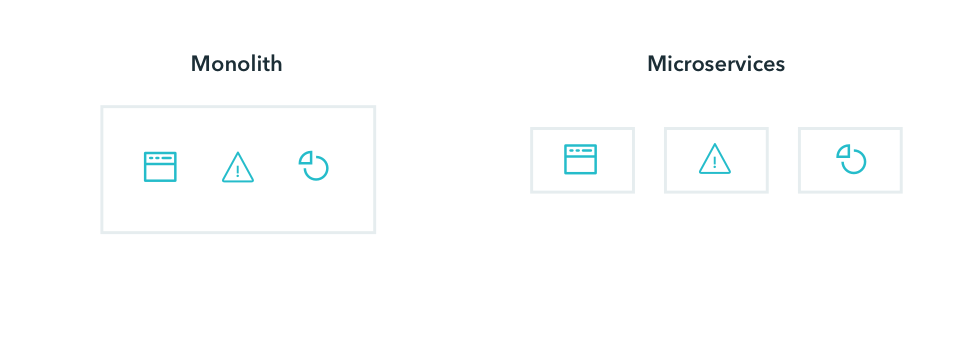
\includegraphics[width=10cm]{Mono_Micro.png}
	\centering
	\caption{Een monolithic vergeleken met een microservice. \textcite{Benetis2016a}}
\end{figure}


Een voorbeeld van een algemene architectuur is te zien op figuur 2.3.
\begin{figure}[h!]
	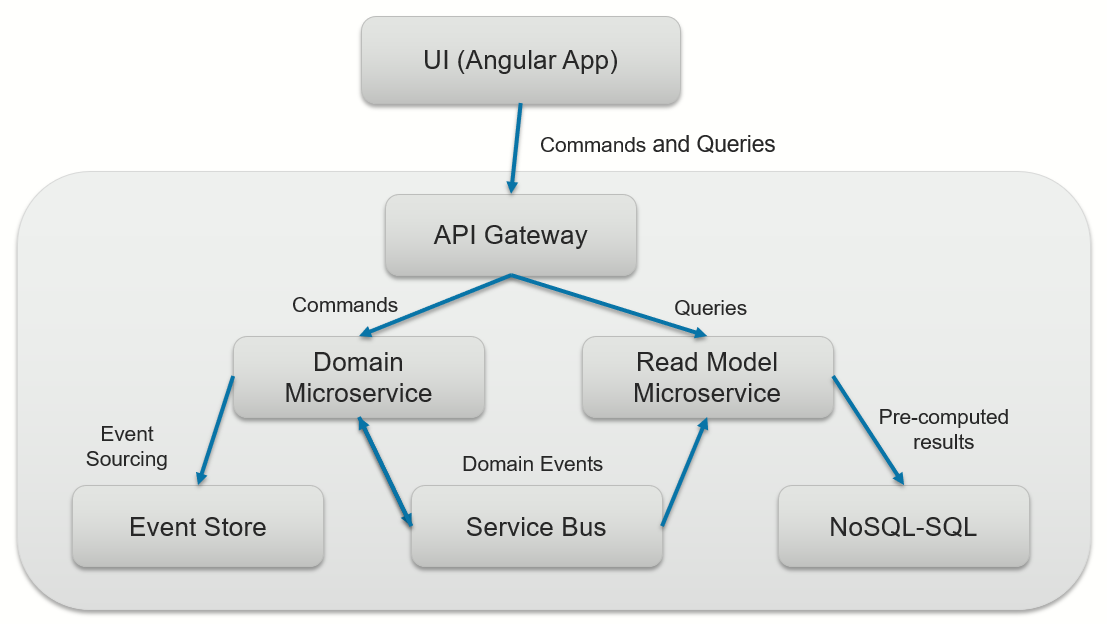
\includegraphics[width=10cm]{algArch.png}
	\centering
	\caption{Een algemene architectuur voor microservices. \textcite{Koukia2018}}
\end{figure}
Deze afbeelding zal later uitgelegd worden.


\subsection{Het belang van microservices}
Microservices zijn van belang wanneer de monolithic architectuur niet meer optimaal werkt. Microservices hebben nauwelijks invloed op het framework als er deeltjes bij gecodeerd worden. Ze kunnen sneller inspelen op de Agile analyse/ontwikkelsmethode. De analyse methode Agile werkt met periodieke opleveringen, die kunnen gaan van twee weken tot een maand. In die periode wordt er gewerkt aan een functionaliteit of een eis van de klant. 
Ervoor zorgen dat de software schaalbaar is, is een belangrijk punt waar microservices goed op inspelen.


Enkele andere redenen om microservices te gebruiken volgens \textcite{Koukia2018}, zijn ook:
\begin{itemize}
	\item Het is gemakkelijker om kleine services te onderhouden. Bij een monolithic is alles één groot geheel. Als daar een deeltje van moet worden aangepast, kan je verdwalen in het geheel. Dit is niet het geval bij microservices, want elke service is afgebakend met een functionaliteit. Bij het aanpassen van een service kan er duidelijk aangetoond worden waar een service begint en eindigt. 
	\item Een microservice kan onafhankelijk gedeployed worden. Eens een microservice klaar is voor gebruik, hoeft er naar niets anders gekeken te worden. Bij het deeltje definitie  werd hier dieper op ingegaan.
	\item Microservices zijn gemakkelijker aan te passen aan nieuwe  technologie. Komt er een nieuwe  technologie uit die kan toegepast worden op een paar microservices, dan moeten enkel die microservices herschreven worden. Dit is anders bij een monolithic; als er een nieuwe  technologie is die kan toegepast worden op verschillende onderdelen van het geheel, moet de gehele architectuur herschreven worden.
	\item Het is eenvoudiger om te schalen. Schalen gebeurt door een microservice te dupliceren. Niet het gehele systeem moet geschaald worden, enkel de nodige microservices moeten gedupliceerd worden. Het dupliceren van een microservice wil zeggen: de microservice kopiëren en in een ander onderdeel gebruiken. Een microservice dat gedupliceerd kan worden, is dat van logging. 
	\item Er is 'no single point of failure'. Faalt er een microservice in het uitvoeren van zijn functionaliteit, dan heeft dit geen invloed op de andere services. Hier werd dieper op ingegaan in de definitie.
	\item Een microservice geeft vrijheid in het kiezen van de programmeertaal. Dit omvat dat elk team kan kiezen in  welke programmeertaal ze de microservices schrijven. Een team is verantwoordelijk voor één microservice. Ze zijn dus gespecialiseerd in die ene service. 
	\item De evolutie en de oplevering van business features is sneller. Dit komt door de onafhankelijkheid van de services. Er kan op hetzelfde moment aan verschillende services gewerkt worden zonder elkaar te beïnvloeden.
\end{itemize}


In de volgende stukken wordt er dieper ingegaan op de authenticatie en authorisatie, het verband met Agile en Devops, het debuggen binnen microservices en de bescherming van microservices.

\subsubsection{De verschillende manieren van bescherming}
'Microservices moeten een doel in de business vervullen. Naast dit, zorgen microservices ervoor dat de bescherming eenvoudiger wordt.', \textcite{RDX2016}.

De term bescherming omvat het volgende: ervoor zorgen dat hackers de applicatie niet kapot maken.
Hackers zijn mensen die inbreken op een applicatie.

Enkele tips om de bescherming van microservices aan te pakken, \textcite{Matteson2017}, \textcite{Silva2017}:
\begin{itemize}
	\item Zorg bij het ontwikkelen van microservices voor coderingsstandaarden die hergebruikt kunnen worden. Door eenmaal een goede code te voorzien, wordt de kans op kwetsbaarheden en gaten in de bescherming kleiner.
	\item Ga na  welke schade er kan toegebracht worden aan een microservice als die zonder bescherming zou worden geüpload.
	\item Maak gebruik van toegangscontroles. Zorg ervoor dat er gewerkt wordt met leesrechten. Een microservice die de aankooporders ophaalt, mag niet aan de verkooporders kunnen.
	\item Gebruik geen beveiligingsprincipes van externen, maar implementeer deze liever in de code van de microservice.
	\item Zorg voor goede documentatie van elke microservice. Dit kan handig zijn bij het ontdekken van een zwak punt in de bescherming. De documentatie kan mogelijke problemen verduidelijken.
	\item Maak een API gateway. De bedoeling hiervan wordt verder nog uitgelegd.
	\item Zorg ervoor dat enkel de API gateway zichtbaar is en dat alle data onleesbaar verzonden wordt. Dit kan gebeuren aan de hand van SSL of TSL. Wat SSL is wordt verder in deze thesis uitgelegd. 
	\item Zorg voor garantie op data privacy. In Europa is de GDPR een  wetgeving die zegt wat er  wel en niet mag gebeuren met persoonlijke data. Daarom is het belangrijk dat er gebruik wordt gemaakt van een beveiligd protocol. Op elk level moet er gezorgd worden voor een correcte beveiliging van de gebruikers hun data. 
	\item Voor het encrypteren van data wordt er best gebruik gemaakt van al bestaande technologieën en niet zelf één uitvinden. De zelf-uitgevonden manier is niet uitgebreidt getest en zijn niet gekend.
	\item Zorg ervoor dat er geen denial of service kan gebeuren. Denail of service komt voor wanneer er heel veel requests naar de applicatie worden gestuurd, waardoor de applicatie faalt. Maak gebruik van throtteling. De term wordt na deze opsomming verder uitgelegd.
	\item Maak gebruik van Cross-site request forgery (CSRF) en Cross-origin resource sharing (CORS) filters. Cross-site request forgery is een poging tot hacken waarbij de eindgebruiker gedwongen wordt om acties te doen terwijl hij geauthenticeerd is. Cross-origin resource sharing laat toe dat er requests van een ander domein kunnen worden gemaakt. 
	\item De API gateway kan goed beschermd zijn maar zorg eveneens voor goede bescherming aan de code. Zorg ervoor dat er niks moet worden gerund als administrator, geef duidelijke namen en maak duidelijke afspraken. Enkel de nodige personen mogen de juiste permissies krijgen. 
\end{itemize}

\textcite{Troisi2019} geeft acht best practices over de bescherming van microservices. 
De best practices:
\begin{itemize}
	\item Het gebruik van OAuth voor gebruikers identificatie en wat de gebruiker kan. OAuth/OAuth2 is een protocol voor authorisatie. Het is een gemak om gebruik te maken van een protocol omdat ze gekend en actief gebruikt worden. Een protocol is een aantal regels om te communiceren tussen computers. 
	\item Gebruik bescherming in de diepte om een prioriteit toe te kennen aan service keys.  Dit kan verwoord worden als bescherming steken in verschillende lagen van een systeem. Er moet worden nagegaan  welke deeltjes het kwetsbaarst zijn en daar dan verschillende lagen van beveiliging op toe te passen. 
	Microservices maken het toepassen van deze methode eenvoudiger. omdat er gefocust kan worden op beveiliging. Het framework maakt het gemakkelijker om de verschillende lagen vast te stellen. Als hackers binnen zijn bij één van de microservices, zijn ze niet binnen in het volledige systeem. 
	\item Schrijf zelf geen krypto code. Er zijn genoeg open source alternatieven. Enkel bij heel uitzonderlijke redenen wordt een eigen krypto code geschreven. 
	\item Update je bescherming tijdig. Als er updates komen in de software van beveiliging, moeten die uitgevoerd worden. Het automatiseren van die updates kan veel  werk besparen achteraf. Dit wordt dan best gedaan bij het creëeren van microservices. Bescherming binnen software is niet langer een nice to have maar een must have. 
	\item Maak gebruik van een firewall met gecentraliseerde controle. Het biedt onder andere meer controle aan de gebruiker. 
	\item Maak gebruik van software om virussen te vinden.
	\item Monitor alles.
\end{itemize}

Throtteling, \textcite{Cavalcanti2018}, is een manier van bescherming wat het volgende beschrijft: 'Throttling is a process used to control the usage of APIs by consumers during a given period.'. Het kan zijn dat de gebruiker heel veel requests stuurt naar de API gateway. Dit kan zorgen voor een bug door een oneindig aantal requests. Om dit te voorkomen kan er een limiet binnen een bepaalde periode opgelegd worden. Bijvoorbeeld als je je toegangscode drie maal fout hebt op je gsm, dan blokkeert die voor een bepaalde tijd. Het systeem dus zo ontwerpen dat het bestand is tegen fouten en falen. Met 'bestand zijn tegen' wordt bedoelt: ervoor zorgen dat bij een bug of een fout, deze goed wordt opgevangen zodat de gebruiker er geen last van heeft. 

Eén van de meer bekende manieren is de API gateway. De verantwoordelijkheden van een API gateway zijn de volgende, \textcite{Siraj2017}:
\begin{itemize}
	\item Het ontvangen van request van gebruikers.
	\item De requests doorsturen naar de correcte microservice.
	\item Het 'antwoord' van de microservice in ontvangst nemen en doorsturen naar de gebruiker.
\end{itemize}
Zoals te zien is op figuur 2.4, is een API gateway het toegangspunt. Om via de API gateway requests te kunnen maken, moet er eerst authenticatie en authorisatie toegepast worden. Meer uitleg hierover in de sectie over authenticatie en authorisatie.
\begin{figure}[h!]
	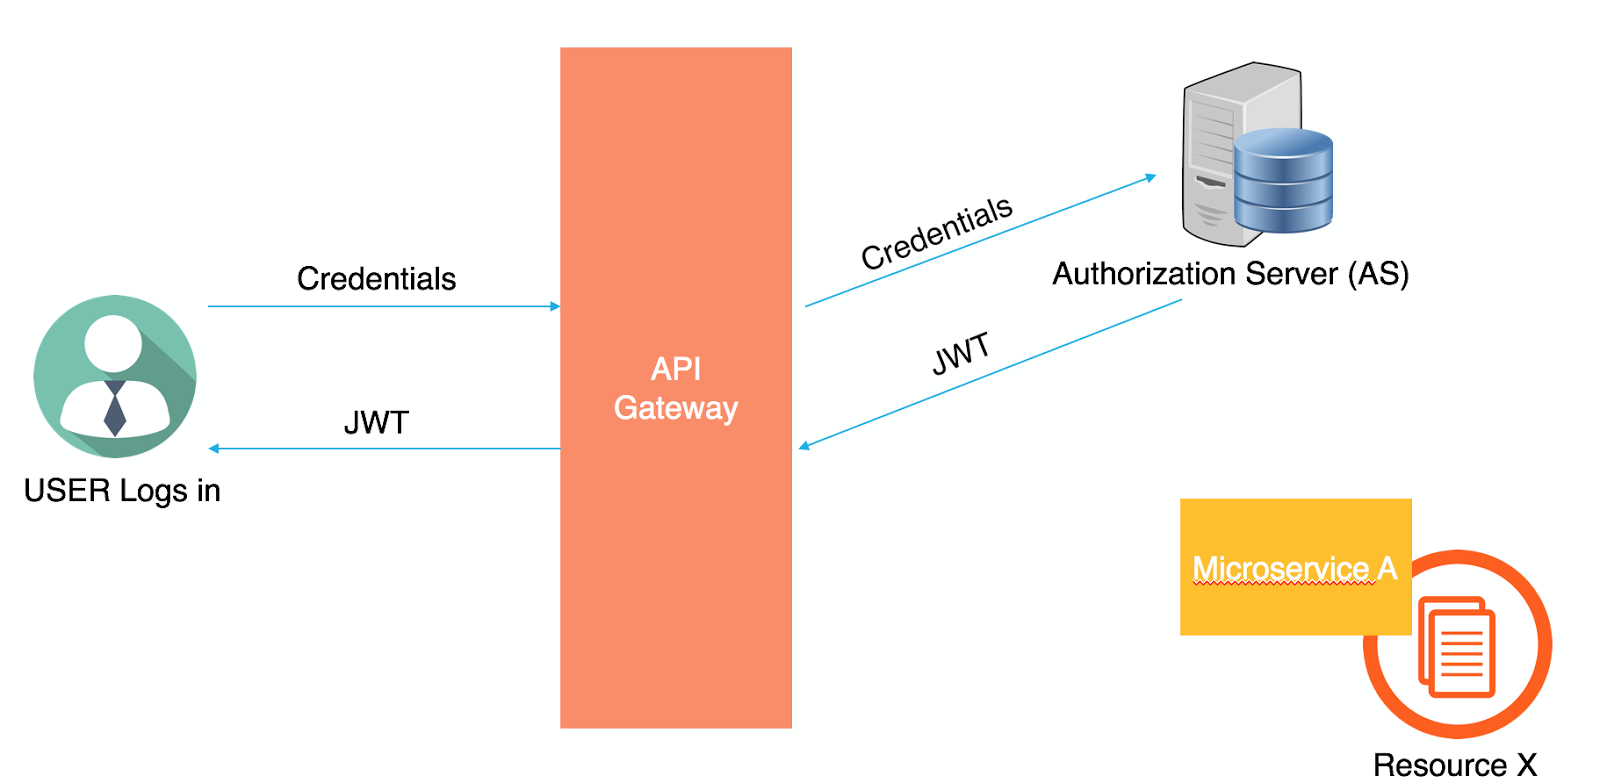
\includegraphics[width=10cm]{apiGateway_facadePattern.png}
	\centering
	\caption{Een voorstelling van API gateway. \textcite{Siraj2017}}
\end{figure}


\subsubsection{Authenticatie en authorisatie}
Een belangrijk aspect van microservices is de authenticatie en de authorisatie.  Het is een moeilijkheid om op een uniforme manier veiligheid, bescherming, authorisatie en authenticatie toe te passen op microservices, \textcite{Ayoub2018}. Authenticatie is het bevestigen van de identiteit van de gebruiker. Dit wordt doorgaans gedaan door middel van een gebruikersnaam en een wachtwoord. Authorisatie is wat je kan doen met een programma. Bijvoorbeeld een beheerder van een site kan meer dan een bezoeker. 
\begin{figure}[h!]
	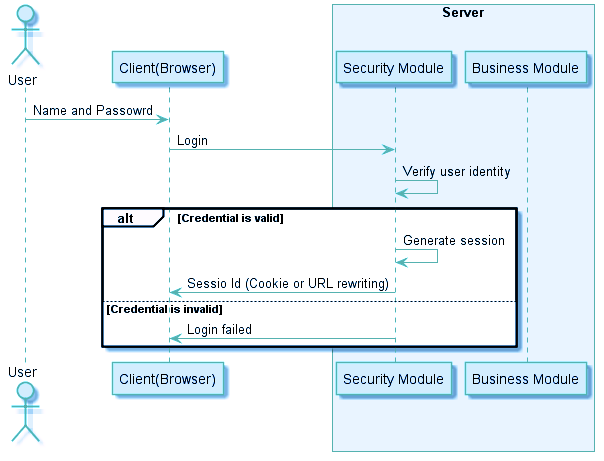
\includegraphics[width=10cm]{monolithic_auth.png}
	\centering
	\caption{Een diagram van authenticatie bij een monolithic. \textcite{Ayoub2018}}
\end{figure}
Zoals te zien is op bovenstaande afbeelding, figuur 2.5, wordt de authenticatie afgehandeld binnen het monlithic proces. Wanneer de gebruiker inlogt, wordt de beveiligingsmodule aangesproken. Deze kijkt of de gebruiker een bekende is, of er al gegevens in de databank zitten. Als het aanmelden gelukt is, wordt er een sessie gecreëerd. Een sessie wordt opgeslagen aan de hand van tokens. Tokens worden op je computer geplaatst door je browser. Het zijn kleine tekstbestanden. De sessie onthoudt wie je bent aan de hand van een ID. Dit zorgt ervoor dat je je niet elke keer opnieuw moet aanmelden als je van pagina verandert.  Elke keer dat de bezoeker van de site iets doet, wordt de sessie ID samen gestuurd met de request. Een request is een aanvraag. Als het ID correct is,  weet de site dat de gebruiker ingelogd is. Bij elke aanvraag wordt de ID meegestuurd voor controle. Op die manier wordt de authenticatie bij een monolithic afgehandeld.
Wanneer er gekeken wordt om authenticatie toe te passen bij microservices, wordt het volgende aangehaald:
\begin{itemize}
	\item In elke microservice moet er authenticatie en authorisatie afgehandeld worden. Het beste wordt dit toegepast op een uniforme manier. Dan gaat men ervan uit dat er in elke microservice een stukje code komt dat hergebruikt wordt. Maar dit zorgt er voor dat elke microservice toch afhankelijk is. Bij het uitkomen van een nieuwe  versie, moet dit deeltje dan  weer geüpdate worden. Dit heeft invloed op de flexibiliteit van het framework.
	\item 'Single responsibility' zijn twee woorden die microservices mooi omschrijven. Een microservice omvat een stukje business logica. De algemene logica van authenticatie en authorisatie mag niet in een microservice gegoten worden. 
\end{itemize}
In het algemeen zijn authenticatie en authorisatie een complex onderdeel van microservices.
Er zijn vier oplossingen volgens \textcite{Ayoub2018}:
\begin{itemize}
	\item Distributed session manangement,
	\item client token,
	\item single sing-on, 
	\item client token with API gateway.
\end{itemize}
Distributed Session management is de eerste oplossing. Het managen van een sessie over microservices kan op verschillende manieren aan de hand van Sticky sessions. Dit houdt in dat alle requests van één gebruiker naar dezelfde server worden gestuurd waardoor men ervan kan uitgaan dat de gebruikte data van die specifieke gebruiker is. Of men kan dit toepassen via session replication. Dit houdt in dat alle instanties de sessie data synchronizeren. Deze manier van toepassen heeft als nadeel dat er veel overhead aanwezig zal zijn op het netwerk. Een andere methode is centralized session storage. Deze omvat dat bij het aanspreken van een microservice, deze de gebruikersdata ophaalt van op een gedeelde plaats. 
Een andere manier om authenticatie en authorizatie toe te passen, is via een client token. Een token wordt gebruikt om aan te tonen dat je echt de gebruiker bent. Een token wordt bijna altijd onleesbaar gemaakt. Het klinkt bijna hetzelfde als een sessie. Het verschil is dat een sessie op de server centraal wordt bijgehouden. Een token wordt bijgehouden door de user zelf.
Naast de Distributed session management en client token is er nog single sign-on. Na een enkele aanmelding kan de gebruiker alle microservices gebruiken binnen de applicatie. 
Een andere manier is een client token with API gateway. Deze manier is gebaseerd op de client token maar nu is er een API gateway toegevoegd aan het begin van een externe request. Dit zorgt ervoor dat het framework niet zichtbaar is voor de buitenwereld. 

Door de API Gateway to combineren met JSON  web Tokens is er meer mogelijkheid om te schalen,\textcite{Siraj2017}. 
\begin{enumerate}
	\item De gebruiker meldt zich aan.
	\item De API gateway stuurt de request door naar de server die instaat voor de authenticatie.
	\item Is de authenticatie goedgekeurd, wordt er een JWT token teruggestuurd naar de gebruiker. Meer uitleg over de JWT na dit proces.
	\item Bij de volgende request wordt de token automatisch meegestuurd met de request.
	\item Een andere server kijkt bij elke request naar de token om na te gaan of de gebruiker de juiste authorisatie heeft. 
\end{enumerate}
De token vervalt na een bepaalde tijd. Er kan gekozen worden om deze automatisch te laten verlengen. Hier wordt niet verder op ingegaan. 

De definitie van JSON  web Token, \textcite{Stecky-Efantis2016}: 'A JSON  web Token (JWT) is a JSON object that is defined in RFC 7519 as a safe way to represent a set of information between two parties. The token is composed of a header, a payload, and a signature.'. Het diagram te zien in figuur 2.6 is een schematische voorstelling van hoe een JWT token wordt gegeven aan een gebruiker.
\begin{figure}[h!]
	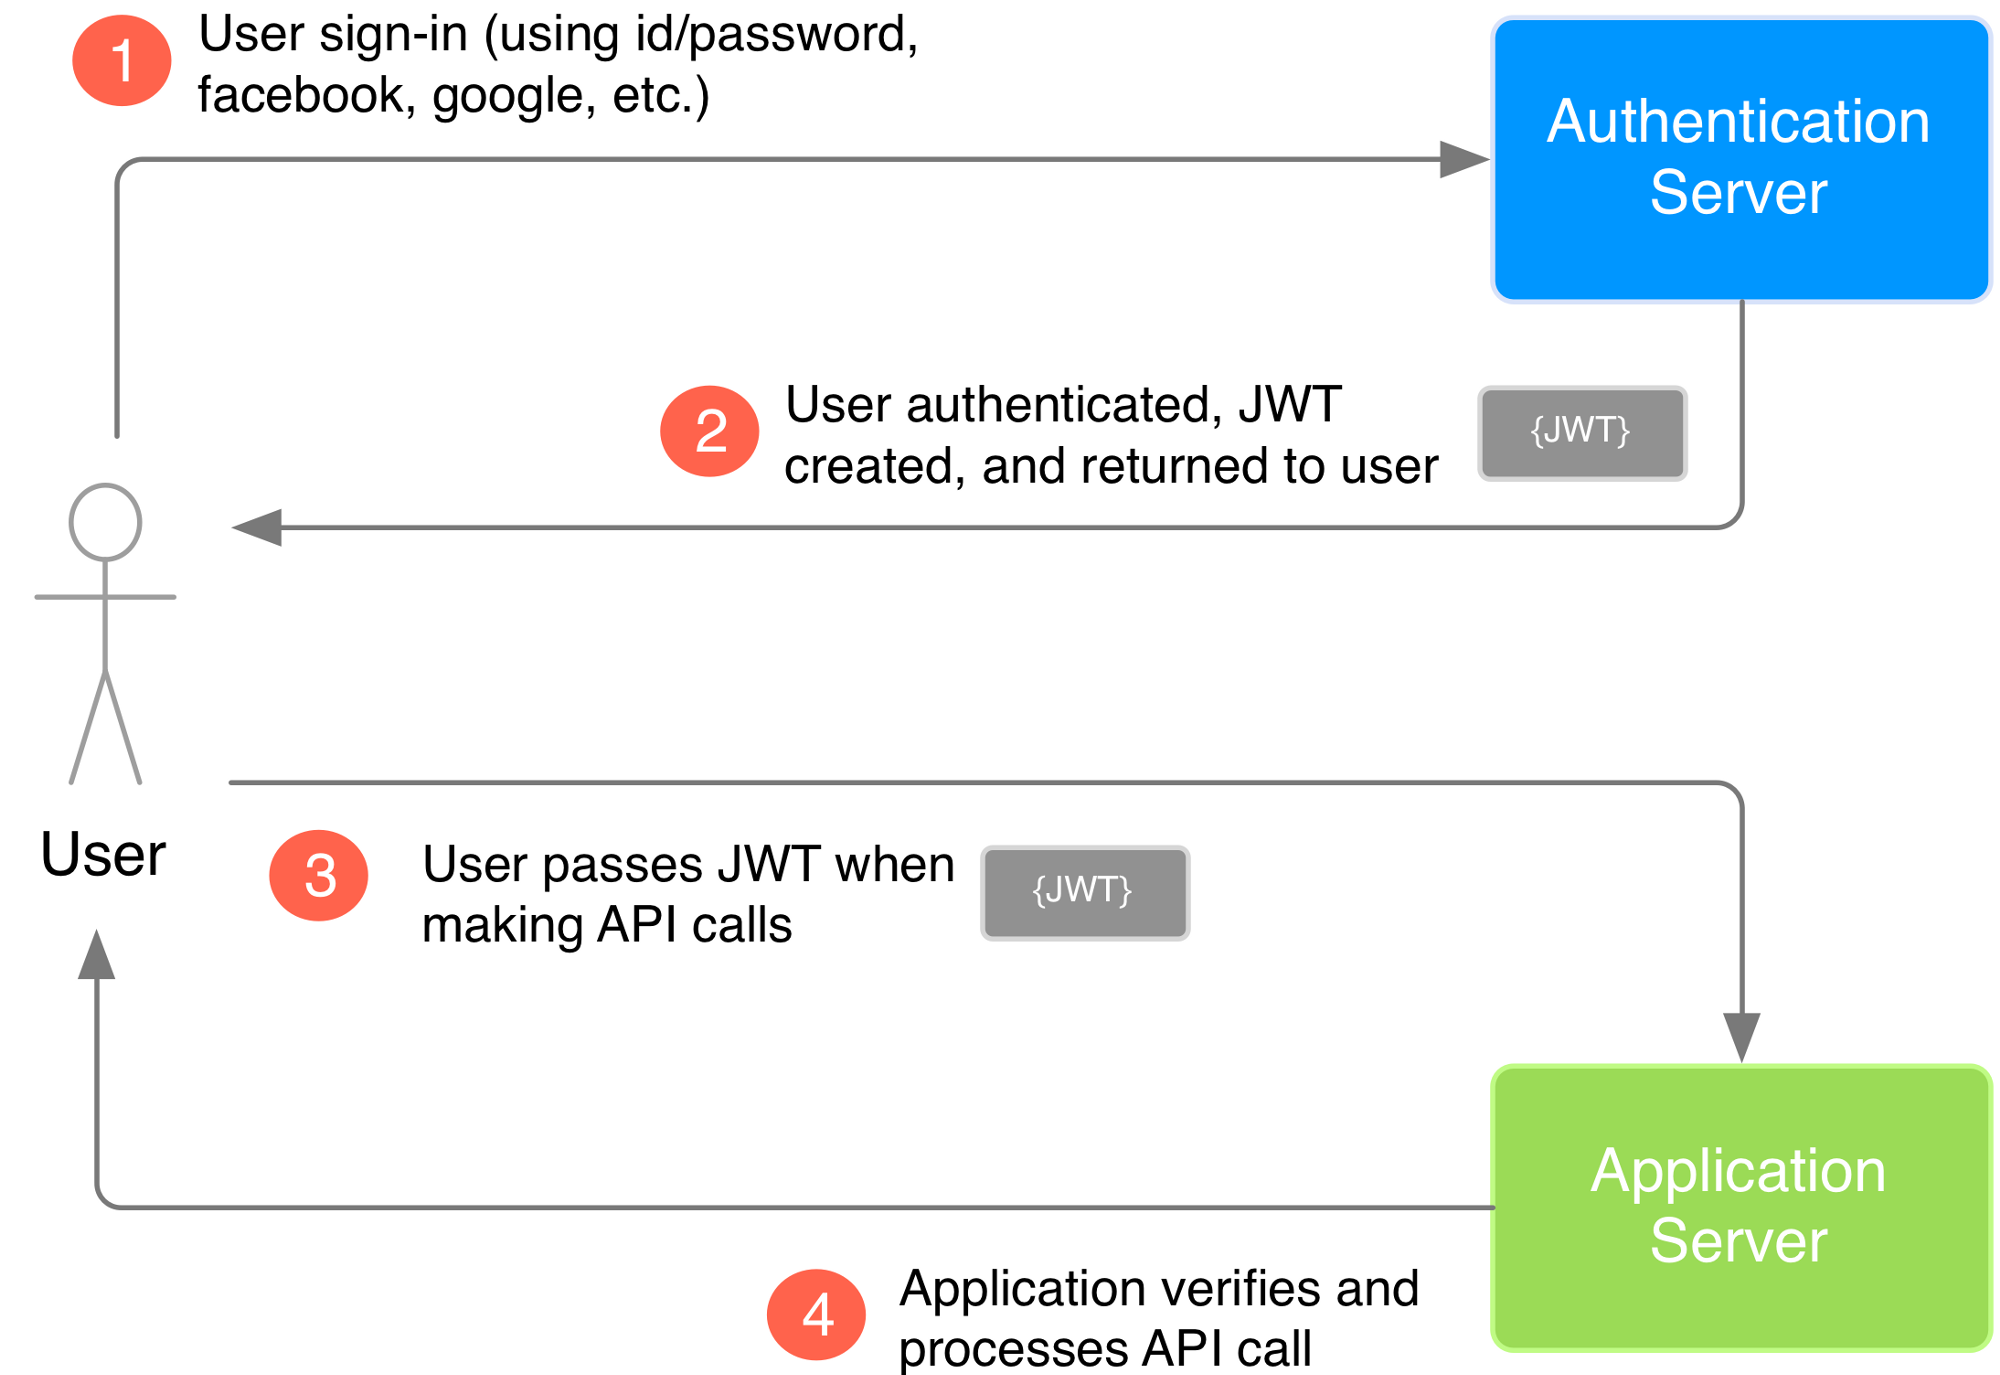
\includegraphics[width=10cm]{jwt.png}
	\centering
	\caption{Een schematische voorstelling van het geven van een JSON  web Token. \textcite{Stecky-Efantis2016}}
\end{figure}
Het proces gaat als volgt:
\begin{enumerate}
	\item Aanmelden op een platform. Bijvoorbeeld aanmelden op Facebook, Twitter, Instagram of Google.
	\item De authenticatie server stuurt een JWT terug.
	\item Bij het maken van requests wordt de token meegestuurd.
	\item De microservice kijkt dan of de gebruiker het recht heeft om deze microservice/functie te gebruiken.
\end{enumerate}


\subsubsection{Verband met Agile en DevOps}
Microservices komen uit dezelfde ideologie als Agile en DevOps. DevOps is een contaminatie  van development en operations. Bij deze methode ligt de nadruk op de samenwerking en communicatie tussen verschillende partijen. Hier zijn de partijen de software engineers en andere IT-specialisten. Deze ideologie omvat het volgende: het afbreken van een kleine, traag evoluerende architectuur of monolithic en deze in microservices steken.

DevOps heeft volgende definitie: 'DevOps is a methodology that enables developers and IT Ops to work closer together so they can deliver better quality software faster', \textcite{Morgan2019}. Met DevOps probeert men de productie zo goed mogelijk na te bootsen. Net zoals bij Agile, zorgt DevOps ervoor dat de software in kleinere delen wordt opgesplitst om opnieuw op kortere periodes deeltjes software op te leveren. Dit is iets waar microservices in terug te vinden zijn. Verschillende DevOps teams kunnen dus tegelijkertijd aan microservices  werken.

Enkele voordelen van de combinatie microservices en DevOps:
\begin{itemize}
	\item Meer opleveringen van software op kortere periodes.
	\item Betere kwaliteit van de code.
	\item Software kan hergebruikt worden.
	\item Een hoger level van automatisatie.
\end{itemize}

Microservices en DevOps vullen elkaar aan op volgende vlakken, \textcite{Mulesoft2019}:
\begin{itemize}
	\item Deployability: Microservices bemoedigen het gebruik van Agile omdat het eenvoudiger is om periodiek op te leveren. 
	\item Reliability: Een fout binnen een microservice heeft enkel effect op die microservice. 
	\item Availability: Het opleveren van nieuwe  deeltjes neemt niet veel tijd in beslag. De gehele applicatie zal niet lang offline zijn.
\end{itemize}




\subsubsection{Het monitoren van microservices}
Logs zijn records binnen een databank die weggeschreven worden terwijl de applicatie draait. Metrics zijn numerieke waarden die kunnen geanalyseerd worden. Metrics zijn terug te vinden op volgende niveau's van een applicatie, \textcite{Wasson2018}:
\begin{itemize}
	\item Node-level: Dit bevat de gegevens van de CPU, het geheugen, netwerk en de harde schijf. 
	\item Applicatie: Hier kunnen metrics bijgehouden worden om het gedrag van de service te begrijpen. Gegevens die bijgehouden kunnen worden zijn het aantal HTTP requests, de vertraging, de lengte van een bericht...
	\item Dependent service: Bij interactie met een externe service kijken hoe lang deze nodig heeft om te reageren. 
\end{itemize}


Het monitoren of loggen van microservices houdt in dat er bijgehouden wordt hoe een microservice zich gedraagt. Er wordt bijvoorbeeld bijgehouden hoe snel de data wordt opgehaald uit de databank. Monitoren vormt dus een belangrijk onderdeel bij het lokaliseren van problemen. \textcite{Ananthasubramanian2018}.


De verschillende tools om te debuggen, \textcite{Swersky2019}:
\begin{itemize}
	\item Logging frameworks: Het is een open-source oplossing. Er zijn verschillende opties; bij het kiezen wordt er best rekening gehouden met volgende punten:
		\begin{itemize}
			\item De netheid van de code. Is de logging code gemakkelijk te lezen?
			\item Wordt de performance beïnvloedt?
			\item Is het framework voor logging al gekend bij het team?
		\end{itemize}
	\item Logging databases: Log data wordt gebruikt voor het capturen van events. Logs worden nooit aangepast en worden gesorteerd op datum en tijd. 
\end{itemize}



Bij microservices wordt elke microservice gelogd. Bij een fout moet er gekeken worden naar alle betrokken microservices en naar alle logs van die service. Om logging toe te passen, wordt er aangeraden om libraries te gebruiken. Enkele best practices, \textcite{Melendez2018}, \textcite{Eyee2018}, \textcite{Timms2018}:
\begin{itemize}
	\item Vermijd dat logs in bestanden worden opgeslagen. Logs zijn streams van een flow. Het geeft  weer wat er precies gebeurd is in een flow.
	\item Microservices hoeven niet te weten waar de logs naartoe gaan. Zo kan de bestemming van het  wegschrijven van de logs veranderd worden zonder dat elke microservice ervoor aangepast moet worden.
	\item De logging moet werken voor alle verschillende codeertalen. Er moet niets worden aangepast bij de configuratie files van het logging systeem.
	\item Geef elke request een uniek ID. Zo kan de request snel teruggevonden worden bij falen. Of bij het zien van een fout kan er snel achterhaald worden  welke request er in fout is gegaan. 
	\item Laat het antwoord een uniek ID meesturen. Als de gebruiker dan een fout krijgt, kan er achterhaald worden waar de teruggestuurde fout vandaan komt. De administrators kunnen dan de details van de fout bekijken.
	\item Een oplossing is om alle logs  weg te schrijven naar een centrale databank. Zo kan het hele pad van de fout snel en eenvoudig teruggevonden worden. Het duurt langer om verschillende fouten aan elkaar te linken als de logs in de datastore van de microservice worden opgeslagen. Bij het opslaan op één plaats worden fouten sneller aan elkaar gelinkt. Het  wegschrijven naar een plaats is tegen het principe van microservices. Binnen die enkele database met alle logs kan er gezocht worden op fout, microservice, tijdstip...  Het volgen van een gebruiker zijn traject binnen de applicatie is eenvoudiger. Bij een fout kan er gekeken worden naar de acties die er op voorhand zijn gemaakt. 
	\item Zorg voor structuur in de log data. Gebruik een algemene format zoals JSON of XML om een structuur te creëeren in de logs. 
	\item Geef iedere request een context.  De oorzaak van de fout kennen, is belangrijk om ervoor te zorgen dat de fout zich niet zal herhalen. Volgende velden zouden zeker in de log terug te moeten vinden zijn:
		\begin{itemize}
			\item Dag en tijd.
			\item Stack errors.
			\item De naam van de service, om de logs te linken aan microservices.
			\item In  welke functie de fout is ontstaan.
			\item De naam van de externe service waar er interactie mee is geweest.
			\item Het IP adres van de server en van de gebruiker zijn requests. 
			\item De browser waaruit de gebruiker de request stuurde.
			\item De HTTP code om later alerts te creëren. 
		\end{itemize}
	\item Overweeg om de logs naar een lokale databank  weg te schrijven. Elke oplossing heeft zijn voor- en nadelen. Het  wegschrijven over HTTP naar de cloud kan zorgen voor meer verkeer op het netwerk. De bandbreedte kan bij belangrijke microservices verminderd worden. 
	\item In het begin wordt er best veel gelogd. Later kan beslist worden om enkele parameters niet meer te loggen.
\end{itemize}



\subsection{De voordelen en nadelen van microservices}
Het gebruik van microservices zorgt ervoor dat de architectuur flexibeler wordt.  Dankzij microservices is het hermodeleren, implementeren van nieuwe  technologieën... eenvoudiger.
Kleinere deeltjes zijn gemakkelijker te documenteren. Ook de snelheid van microservices zijn een groot pluspunt. Microservices reageren sneller omdat ze kleine, onafhankelijke services zijn. Ze moeten geen onnodige stappen maken om de  wens van de klant te vervullen. 

\textcite{Watts2018} en \textcite{Benetis2016} geven nog andere voordelen van een microservice. Een developer is onafhankelijk, ze moeten niet wachten een andere developer. Dit is een gevolg van het feit dat microservices onafhankelijk zijn. Microservices zijn sneller en gemakkelijker te deployen.

Het scalen van een microservice is veel eenvoudiger. Omdat dat microservices minder resources nodig hebben dan een volledige monolithic. Resources zijn hulpbronnen onder andere protocollen, programmeerstandaarden... 

Binnen een monolithic zijn deeltjes afhankelijk van elkaar om goed te kunnen functioneren. Nog een voordeel: bij het falen van een microservice zal de ander geen last ondervinden. 

Een eerste nadeel is dat de scope gedetailleerder moet zijn omdat het project ingedeeld is in kleinere requirements. Als gevolg van zijn de teams kleiner en een teamlid kan niet zomaar vervangen worden omdat elk team een bepaalde specialisatie heeft.

\textcite{Koukia2018} drukt ons op het feit dat het onderhouden van microservices veel werk vraagt. Het is een nieuwe technologie en het team moet up to date blijven over die technologie. Dit is een van de redenen waarom sommigen bij een monolithic blijven. De complexiteit binnen monolithic is gekend. De developers zijn et gewoon om met die complexiteit te werken en er fouten uit te halen. Daarom lijkt de chaos bij microservices soms groter dan bij een monolithic.

\section{Microservices integration patterns}
Hierboven werd uitgelegd wat microservices zijn. Het zijn kleine, onafhankelijke services die aan business requirements voldoen. Maar die moeten met elkaar kunnen communiceren, taken uitvoeren, data updaten en elkaar kunnen raadplegen. Om ze met elkaar te laten communiceren, moeten ze op een gestructureerde manier geintegreerd worden in de applicatie. Gestructureerd integreren kan a.d.h.v. onderstaande patterns:
\begin{itemize}
	\item Anti-patterns
	\item Communicatie tussen de microservices
	\item Data integration
	\item Extract, transform en load (ETL)	
\end{itemize}

In het derde hoofdstuk zal 1 van de meerdere bovenstaande patterns theoretisch toegepast worden op het order-to-cash proces. Het order-to-cash proces zal verder uitgelegd worden in deel 2.3.
\subsection{Anti-patterns}
Een anti-pattern is het implementeren van microservices op een ongestructureerde manier zonder grondig onderzoek te doen. 
Anti-patterns ontstaan bij een ongeplande overschakeling naar microservices.  Anti-patterns komen vaker voor dan een gestructureerde microservice architectuur omdat ongepland ergens aan beginnen eenvoudiger is dan alles plannen en voorbereiden. Er moet grondig onderzoek gedaan worden naar de verschillende 'microservice integration patterns'. Op welke manier kan de applicatie gestructureerd naar een microservice architectuur veranderd worden?
De meeste mensen hebben niet door dat ze een anti-pattern aan het maken zijn. . 

Er zullen drie anti-patterns besproken worden die kunnen helpen bij het achterhalen ervan. Volgende zullen besproken worden, \textcite{Monson2019}:
\begin{itemize}
	\item Break the piggy bank
	\item Everything micro
	\item We are Agile: The Frankenstein
\end{itemize}
\subsubsection{Break the piggy bank}
Bij een break the piggy bank structuur lijkt de applicatie wat op een spaarvarken. Om van een monlithic applicatie naar een microservice applicatie te gaan, moet de applicatie uit elkaar gehaald worden en opgedeeld worden in kleine delen.  De kleine delen worden omgezet naar microservices. 
In het begin van de verandering naar microservices zal de complexiteit verminderen. Maar  verder in het proces wordt het enkel complexer door de ongestructureerde overgang.
De applicatie is opgedeeld in onderdelen en die onderdelen zijn omgezet in microservices. Bij het samenvoegen van de microservices tot een architectuur, is het mogelijk dat de applicatie een mini-monolithic wordt. Dit komt voor wanneer de services niet opgedeeld worden op basis van functionaliteit maar willekeurig worden samengevoegd zonder op voorhand na te denken.
Dit anti-pattern is het populairst wanneer een monolithic applicatie niet meer houdbaar is. Dit pattern kan goed gebruikt worden als het in combinatie met een ander integration pattern wordt gebruikt.
De figuur 2.7, die dit anti-pattern illustreert, is terug te vinden op pagina 31.
\begin{figure}[h!]
	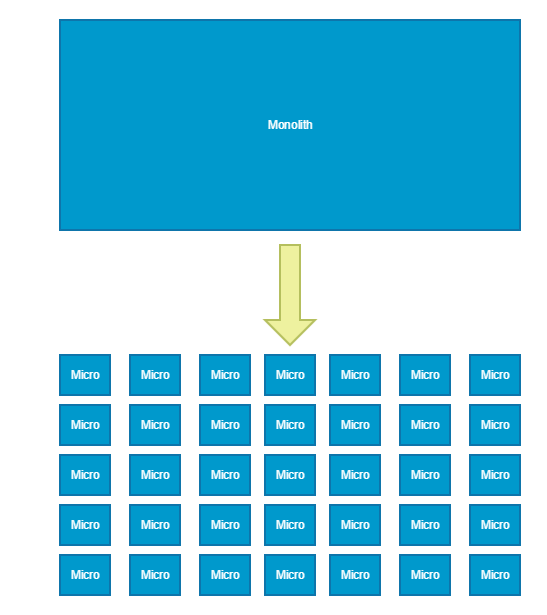
\includegraphics[width=10cm]{breakthepiggybank.png}
	\centering
	\caption{Break the piggy bank, van monolithic naar microservices via anti-pattern \textcite{Monson2019}}
\end{figure}

\subsubsection{Everything micro}
Alles in de applicatie wordt omgezet naar microservices, behalve de databank. De verschillende microservices moeten de data uit een gemeenschappelijke databank opvragen. Deze wordt dan snel de 'bottleneck' in de applicatie. De term 'bottleneck' wordt gebruikt wanneer er een plaats is binnen de applicatie waar alle delen vertraagd worden. Alle aanvragen komen binnen, maar er kunnen er maar enkele verwerkt worden.
Om de data van de databank op te halen, moet 'access control' uitgevoerd worden. Niet alle microservices kunnen tegelijkertijd hun data opvragen en ontvangen.
Dit moet op een gecontroleerde manier, anders is er kans op 'deadlock'. Deadlock komt voor wanneer twee of meerdere services data van de databank willen halen. 
De datastructuur blijft in feite monolithic.
Op het eerste gezicht lijkt dit geen groot probleem. Naast een verhoogd risicoop vertragingen, komt dit anti-pattern met een extra uitdaging: de verandering van de databankschemas bijhouden. Omdat er maar één databank gebruikt wordt, moet elke verandering van elke microservices genoteerd worden. Naast die uitdaging moet bij een verandering in de productiedatabank, de volledige applicatie opnieuw gedeployed worden. Een productie databank is de databank die live gebruikt wordt door klanten. Een voorbeeld van een productie databank: de databank waarmee je communiceert als je op Zalando iets besteld. Een alternatief hiervoor is terug te vinden in 'Data integration'.
Figuur 2.8 illustreert hoe 'everything micro' er kan uitzien. Dit is terug te vinden op pagina 32.
\begin{figure}[h!]
	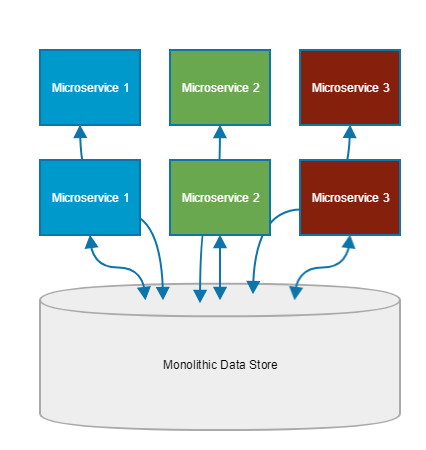
\includegraphics[width=10cm]{everythingmicro.png}
	\centering
	\caption{Everthing micro, anti-pattern met een monolithic databank. \textcite{Monson2019}}
\end{figure}

\subsubsection{We are Agile: The Frankenstein}
Dit anti-pattern ontstaat vaak door de overschakeling van watervalanalyse naar de Agile methodologie. Bij watervalanalyse wordt er één groot plan opgesteld voor een project. Dat plan wordt uitgevoerd in de hoop dat er geen veranderingen worden doorgevoerd in het project. 
Door de simpliciteit van de omschakeling wordt soms gedacht dat er geen voorbereiding nodig is. 
De meeste teams gaan van de waterval methode naar een combinatie van Agile en waterval. 
Het gevolg van een ongestructureerde planning zijn delen die los van elkaar zijn geprogrammeerd en die niet kunnen samenwerken. Ze worden aan elkaar 'genaaid' om samen te werken. Net zoals Frankenstein aan elkaar is genaaid met verschillende onderdelen. De samengevoegde onderdelen moeten de databank delen. Telkens er een nieuwe functionaliteit moet toegevoegd worden, wordt de architectuur complexer en moeilijker om te deployen. 
Omdat de architectuur een ongestructureerd samenhang is van losse onderdelen, kan de applicatie op lange termijn transacties doen waarvoor die niet geprogrammeerd is. 
De mogelijkheid bestaat dat de applicatie gewoon uit elkaar valt door de slechte architectuur en de chaos die er is. 
De figuur 2.9 geeft een duidelijker beeld van deze methode, de afbeelding is terug te vinden op pagina 33.
\begin{figure}[h!]
	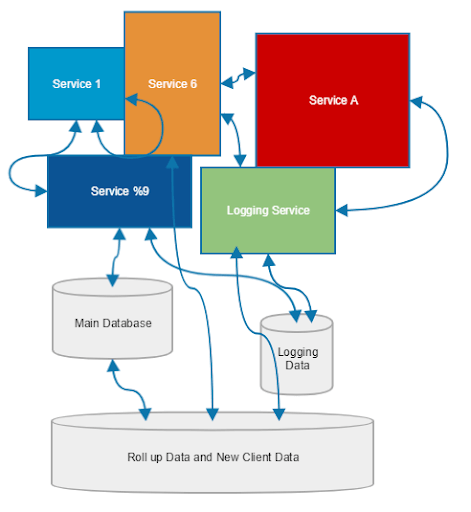
\includegraphics[width=10cm]{frankenstein.png}
	\centering
	\caption{The Frankenstein, anti-pattern waarbij de microservices bij elkaar zijn gevoegd zonder samenhang. \textcite{Monson2019}}
\end{figure}



\subsection{Communicatie tussen de microservices}
Er zijn verschillende manieren om microservices te laten communiceren met elkaar. 
De microservices kunnen elke microservice kennen die ze nodig heeft, maar dit maakt de gehele architectuur complexer. Zoals in afbeelding 2.10 te zien is (pagina 33), zorgt deze manier van communicatie voor een chaotische architectuur.
\begin{figure}[h!]
	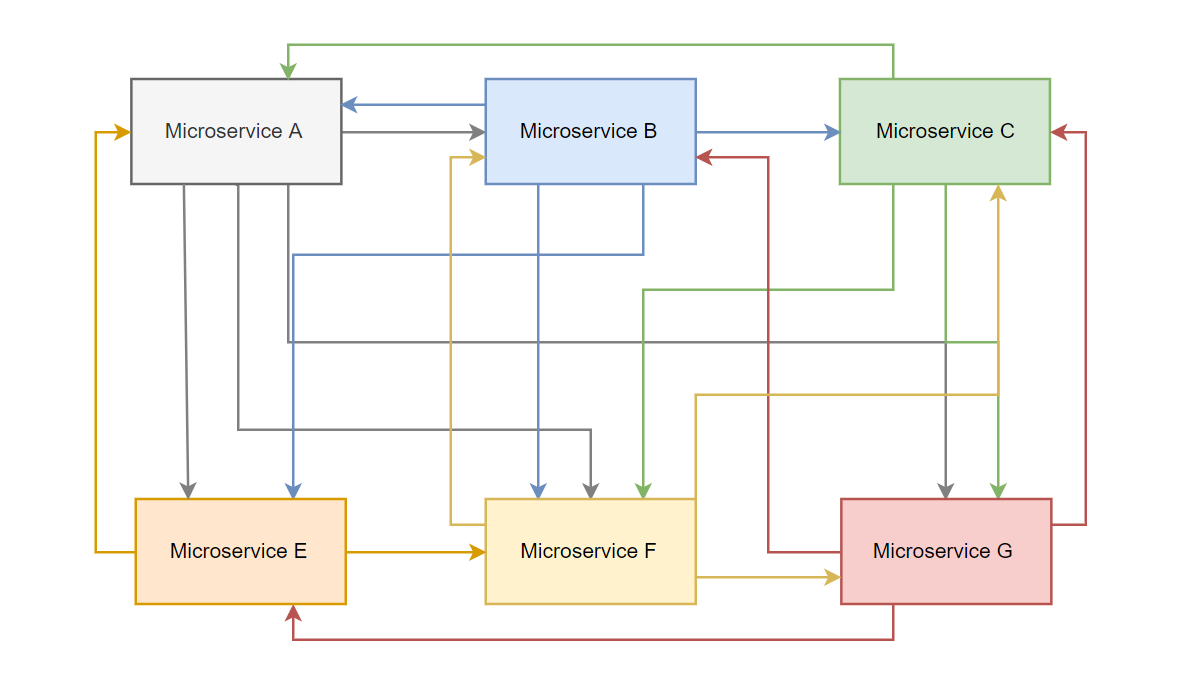
\includegraphics[width=10cm]{chaos.PNG}
	\centering
	\caption{Een architectuur waarbij de microservices elkaar direct kennen om informatie met elkaar te delen.}
\end{figure}

Afbeelding 2.10 illustreert dat de microservices niet meer onafhankelijk zijn en een mini-monolithic vormen. Om ervoor te zorgen dat de microservices onafhankelijk blijven, kan er messaging toegepast worden, \textcite{Solance2018}. Messaging is een manier van communiceren om business entiteiten up te daten, waarbij een 'message broker' gebruikt wordt. Een 'message broker' is de logica die de berichten van een microservice naar een andere stuurt zonder dat ze elkaar moeten kennen. Het meest gekende patroon hiervoor is publish-subscribe pattern. Deze wordt weergegeven in afbeelding 2.11.
\begin{figure}[h!]
	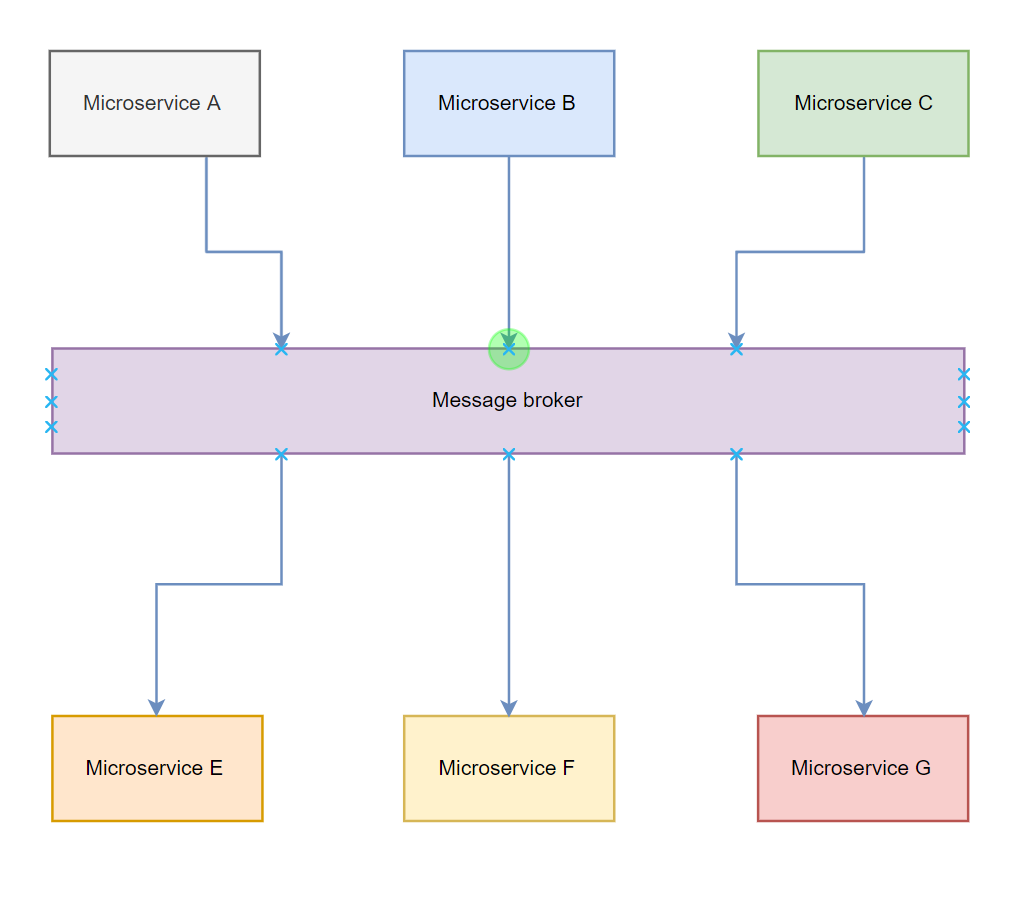
\includegraphics[width=10cm]{messaging.PNG}
	\centering
	\caption{Een architectuur waarbij een message broker als communicatiemiddel wordt gebruikt.}
\end{figure}
In de 'message broker' heeft elke microservices zijn queue. De queue is een wachtrij waar berichten worden opgeslagen. De berichten worden verwijderd van de queue eens ze gelezen en opgehaald worden. 
Een microservice stuurt een bericht naar de 'message broker' en moet zich verder niks van het bericht aantrekken. De 'message broker' zorgt ervoor dat het bericht bij de juiste microservice(s) wordt afgeleverd. De uiteinden kennen elkaar niet en communiceren volledig onafhankelijk van elkaar.
Dit is asynchroon communiceren.

De tegenhanger van asynchroon is synchroon communiceren, \textcite{Gupta2018}, \textcite{Jackson2016} en \textcite{Shore2016}.
Synchroon communiceren omvat dat de verzender wacht op het antwoord van de ontvanger. De verzender vraagt iets, data of informatie, aan de ontvanger dan zal de verzender wachten tot de ontvanger antwoord. Verwoord met microservices: microservice A vraagt aan microservice B informatie of data maar A zal wachten op een antwoord van B wat als gevolg heeft dat ze niet meer onafhankelijk zijn van elkaar. Omdat synchroon communiceren een mini-monolithic, wordt er niet verder op ingegaan. Deze manier van communiceren wordt gebruikt bij Data integration om ervoor te zorgen dat microservices geen andere acties kunnen doen zolang ze nog geen antwoord ontvangen hebben.

\subsection{Data integration}
Data integration wordt door \textcite{Aradhye2018} en \textcite{Kumar2018} uitgelegd. Data integration is een manier om de data van microservices weg te schrijven, op te halen, op te slaan in een databank.
Een opvallende eigenschap aan een monolithic architectuur is de centrale databank. Bij de overgang wordt de databank regelmatig uit beeld gelaten, nochtans is het ook de databank die een grote verandering moet ondergaan. Maar de structuur waarmee er met de data wordt gewerkt, verandert. 
De monolithic databank kan nog gebruikt wordt bij een microservice architectuur, maar  dat brengt veel problemen en obstakels met zich mee. Volgende zijn enkele voorbeelden:
\begin{itemize}
	\item De microservices zijn afhankelijk van dezelfde databank en dus van elkaar. Als meerdere microservices de databank nodig hebben, moeten ze hun beurt afwachten.
	\item Microservices onafhankelijk deployen, is onmogelijk. Een aanpassing heeft invloed op de databank en elke microservice kent de databank. 
	\item Een microservice scalen wordt een moeilijke opgave omdat die vasthangt aan de centrale databank. 
	\item Omdat alle data in één databank wordt bijgehouden, worden de tabellen gigantisch groot en op termijn onhoudbaar en slordig. 
\end{itemize}

Elke microservice heeft zijn eigen databank met data betreffende hun functionaliteit. Hieronder kunnen enkele voorbeelden teruggevonden worden over de voordelen van een microservice met een eigen databank:
\begin{itemize}
	\item De databank bevat enkel de relevante data.
	\item Elke microservice kan apart gedeployed worden. 
	\item Een microservice heeft geen rechtstreekse toegang tot de databank van een andere microservices. 
\end{itemize}

Sommige microservices hebben data van andere microservices nodig omdat hun databank de gewenste gegevens niet kan leveren. De data wordt dan opgevraagd aan de databank waar de gewenste data staat via een de microservice zelf. Dit wordt geillustreerd in afbeelding 2.12, terug te vinden op pagina 34.

Een concreet voorbeeld met klanten data en order data. Op onderstaande afbeelding X is een algemene voorstelling te zien van de microservices die te maken hebben met klanten data en met orders data. 
\begin{figure}[h!]
	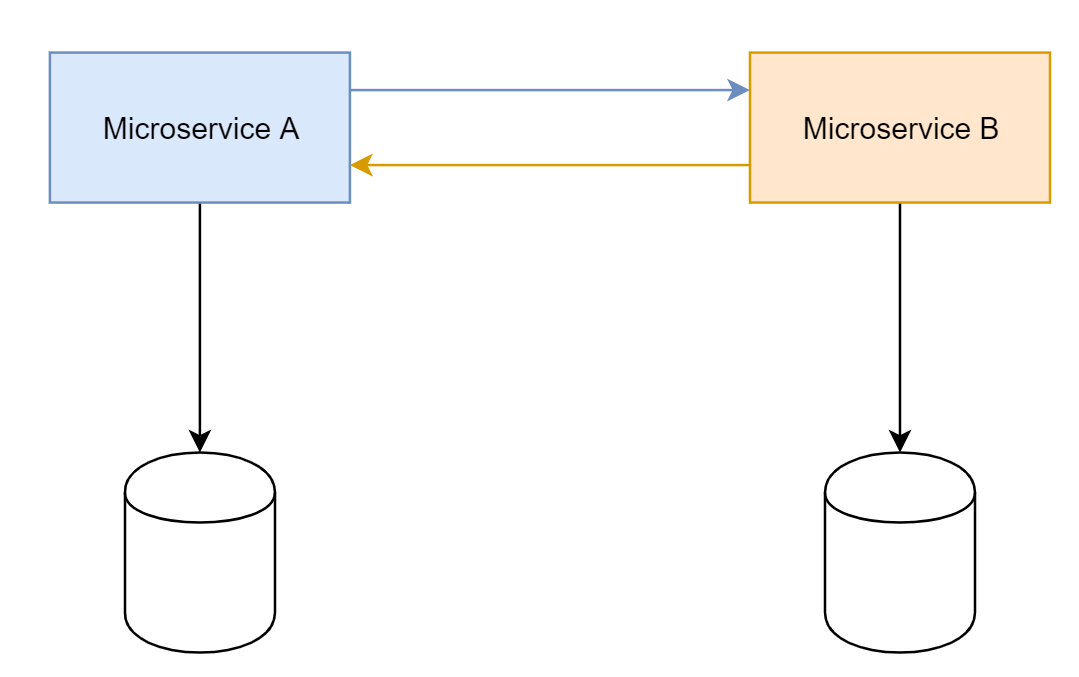
\includegraphics[width=10cm]{db.PNG}
	\centering
	\caption{Hoe een microservice de databank van een andere microservice aanspreekt.}
\end{figure}

De microservice die verantwoordelijk is voor de order data krijgt van een bovenliggende microservice data door om een nieuw order aan te maken. 

\begin{figure}[h!]
	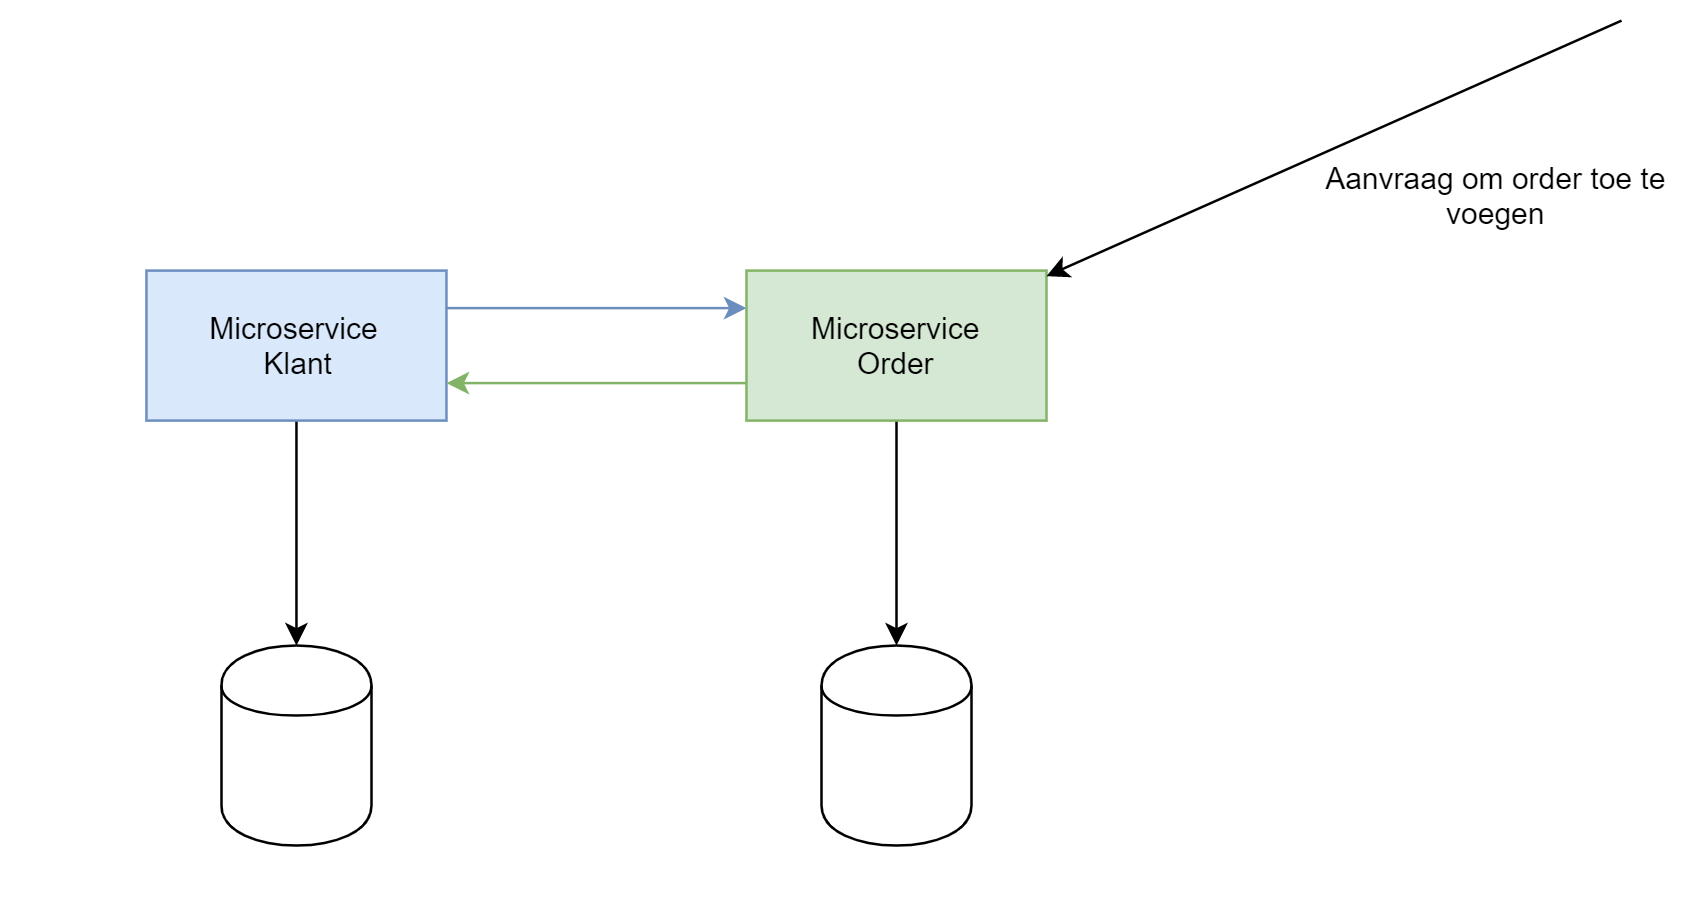
\includegraphics[width=10cm]{db2.PNG}
	\centering
	\caption{De vraag van een ander microservice om een order toe te voegen.}
\end{figure}

De microservice dat het order wil toevoegen, moet het klantnummer opgehaald worden. Dit kan enkel als de microservice die aan de data van de klant kan, aangesproken wordt. De microservice omtrent order data kan niet aan de data van de klant omdat enkel de microservice met de klant data deze kan raadplegen. De microservice omtrent order data spreekt de microservice omtrent klant data aan een vraagt om het klantnummer van een klant met een specifieke naam.

\begin{figure}[h!]
	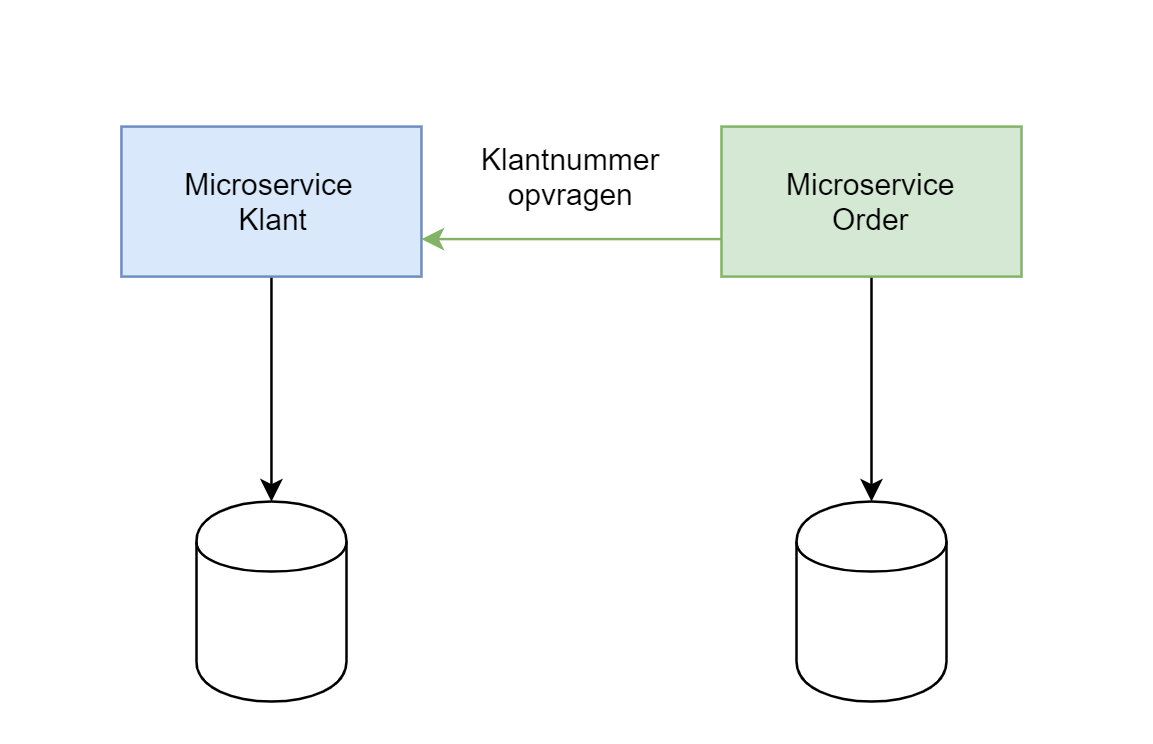
\includegraphics[width=10cm]{db3.PNG}
	\centering
	\caption{Microservice omtrent order data vraagt een klantnummer aan de microservice van klant data.}
\end{figure}

De microservice met klant data krijgt de vraag binnen. Deze reageert met een raadpleging van de databank en stuurt dan een antwoord terug met het klantnummer of een bericht dat deze niet gevonden werd in de databank. 
\begin{figure}[h!]
	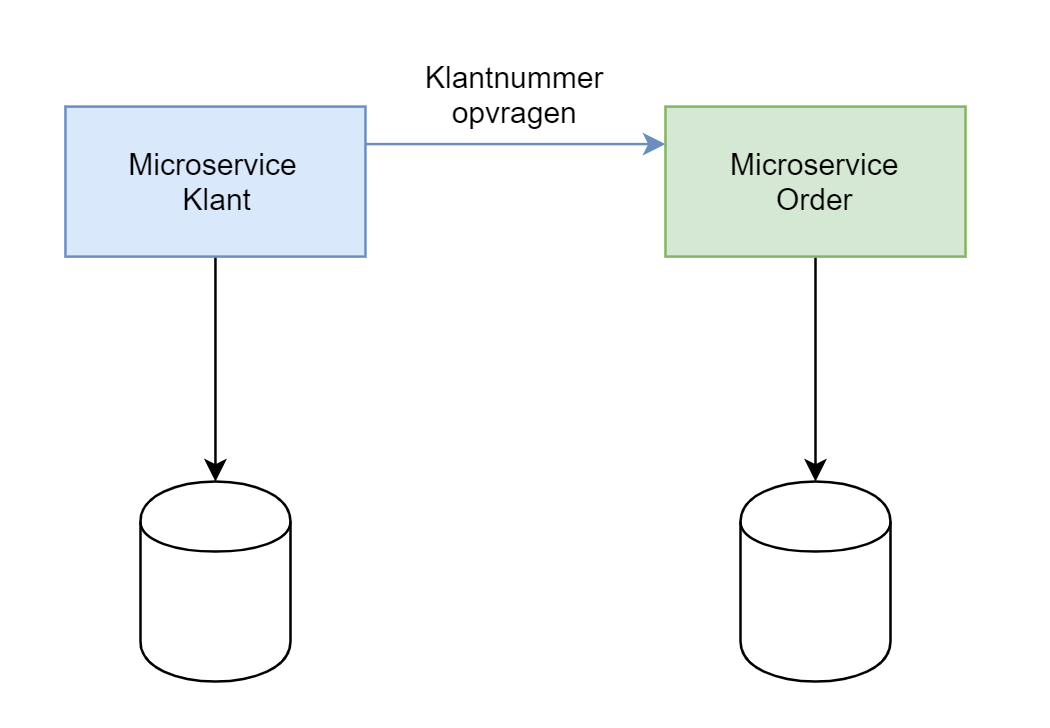
\includegraphics[width=10cm]{db4.PNG}
	\centering
	\caption{Microservice omtrent klant data geeft data terug aan de microservice van order data.}
\end{figure}

Eens de microservice van order data het klantnummer terug krijgt, wordt een nieuw order aangemaakt.
 
De manier waarop microservices gegevens uitwisselen uit hun databank werd beschreven in het vorige deel over 'communicatie tussen de microservices'.
 
Eens de volledige communicatie is uitgedacht, moet er een databank gekozen worden die past bij de micoservices. Het kan zijn dat voor de ene microservice een SQL-databank beter past en voor de ander een NOSQL-databank. SQL en NOSQL zijn soorten databanken. Het verschil tussen de twee is de manier van data opslaan en de manier hoe data wordt opgehaald. Dit wordt niet verder besproken.
 
\subsection{Extract, transform en load (ETL)}
De uitleg over ETL is gebaseerd op artikels van \textcite{Loshin2019}, \textcite{Alley2018}, \textcite{Stich2019}, \textcite{Guru2019} en \textcite{Naveen2016}.

ETL wordt gebruikt  om data te verzamelen, te transformeren en in een andere databank te steken. De data wordt geanalyseerd om het bedrijf een beter beeld te geven van de real-time gebeurtenissen bij bijvoorbeeld marketing. Zo kunnen we te weten komen wat het meest verkocht wordt om 12 uur 's middags. 
ETL bestaat uit drie stappen.
De eerste stap is 'extraction', de data ophalen. De verzamelde data komt niet van één databank maar wordt opgehaald uit verschillende bronnen. Die bronnen zijn databanken die online informatie bevatten over het gedrag van die klant. Belangrijk is dat het verzamelen van de data, de werking van de originele databank niet mag beïnvloeden.
Na het verzamelen van de data, wordt die getransformeerd en gefilterd om enkel de nodige data te verkrijgen. Er wordt meer data verzameld dan nodig is, daarom is het belangrijk dat data gefilterd wordt.
Die data wordt ingeladen in een datawarehouse. Een datawarehouse is een databank waar men data analyseert en logica gebruikt. De business legt op welke analyse er moet gebeuren. De uitkomst van deze analyse kan gebruikt worden binnen het bedrijf of kan gebruikt worden voor artificiële intelligentie.  

\begin{figure}[h!]
	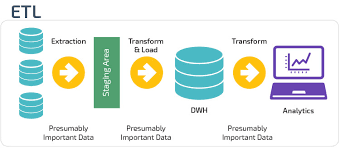
\includegraphics[width=10cm]{etl.PNG}
	\centering
	\caption{Hoe het ETL proces eruit ziet. \textcite{Panolapy2019}}
\end{figure}


\section{Order-to-cash proces in SAP}
\subsection{Definitie}
Het OTC proces is het proces dat begint bij het plaatsen van een order en eindigt bij het betalen van de facturatie en de analyse van de gegevens verzameld tijdens dit proces. Deze worden gebruikt om de verkoop van producten goed te laten verlopen binnen het bedrijf.

Order management is de eerste stap in het proces. Dit begint wanneer de klant een order plaatst. Bijvoorbeeld: ik bestel schoenen op Zalando. Dit deel van het proces moet geautomatiseerd zijn om het proces zo vlot mogelijk te laten verlopen. Als dit deel van het proces niet goed opgezet  is, dan kan het snel slecht gaan. Bijvoorbeeld: orders zitten dubbel in de databank.

Na het plaatsen van een order, wordt de klant gecontroleerd. Credit management: dit moet ervoor zorgen dat er minder problemen zijn op het einde van het proces. Credit management houdt in dat men kijkt naar hoe het betalingsgedrag van de klant is. Zijn er nog openstaande facturen, betaalt de klant pas na enkele aanmaningen? Door dit gedeelte te automatiseren, kan er bespaard worden op personeel en geld. Als er toch dieper moet gekeken worden naar het betaalgedrag van een klant, kan dit doorgestuurd worden naar een fysieke werknemer. Op deze manier moet het betaalgedrag van een paar klanten gecontroleerd worden, i.p.v. alle klanten die een order plaatsen.
 
De klanten die een goed betaalgedrag vertonen, worden doorgestuurd naar de volgende stap: order fulfillment. In deze stap wordt het order samengesteld en uit de rekken gehaald. Bij het verkopen van een product moet de voorraad automatisch aangepast worden. 

Eens de producten van het order samengebracht zijn, gaat  men  over naar order shipping. Dit is de verzending van de goederen. Hierbij wordt de tijd  die nodig is om het product bij de klant te leveren goed opgevolgd om mogelijke vertragingen op te sporen.  

Na het verzenden van de goederen komt de facturatie. Op dit deeltje heeft credit management veel invloed. Doordat de wanbetalers er in stap twee reeds zijn uitgehaald, komen er hier minder problemen voor. Het is belangrijk dat het systeem hier correcte informatie krijgt van de werknemers over order specificaties, de kosten, credit terms, order datum en verzendingsdatum. Op die manier kan ook het facturatiesysteem geautomatiseerd worden.

 Op die manier kunnen vertragingen en fouten geminimaliseerd worden. Eens de factuur is opgestuurd, wordt er een betaling verwacht binnen een afgebakende periode. Het systeem moet dit bijhouden en ervoor zorgen dat er een herinnering gestuurd wordt nog voor de betalingsperiode is afgelopen. Dit valt onder de stap accounts receivable. 
 Wordt een factuur niet betaald binnen de gevraagde periode, dan wordt er een aanmaning gestuurd en wordt dit in het systeem bijgehouden. De klant wordt gecontacteerd en er wordt nagegaan waarom de betaling niet tijdig is gebeurd.
 
Tenslotte komt reporting en data management aan bod. De verzamelde gegevens worden geanalyseerd, waardoor er veel duidelijkheid kan komen over waar het soms verkeerd loopt.

Een OTC proces heeft veel invloed op het succes van een bedrijf, \textcite{Wong2018}. Het proces heeft weerslag op onder meer voorraadbeheer en de financiële afdeling. Het zorgt voor een vlottere interactie met de klant. Er wordt een stabieler beeld gecreëerd van het bedrijf. 
 
\begin{figure}[h!]
	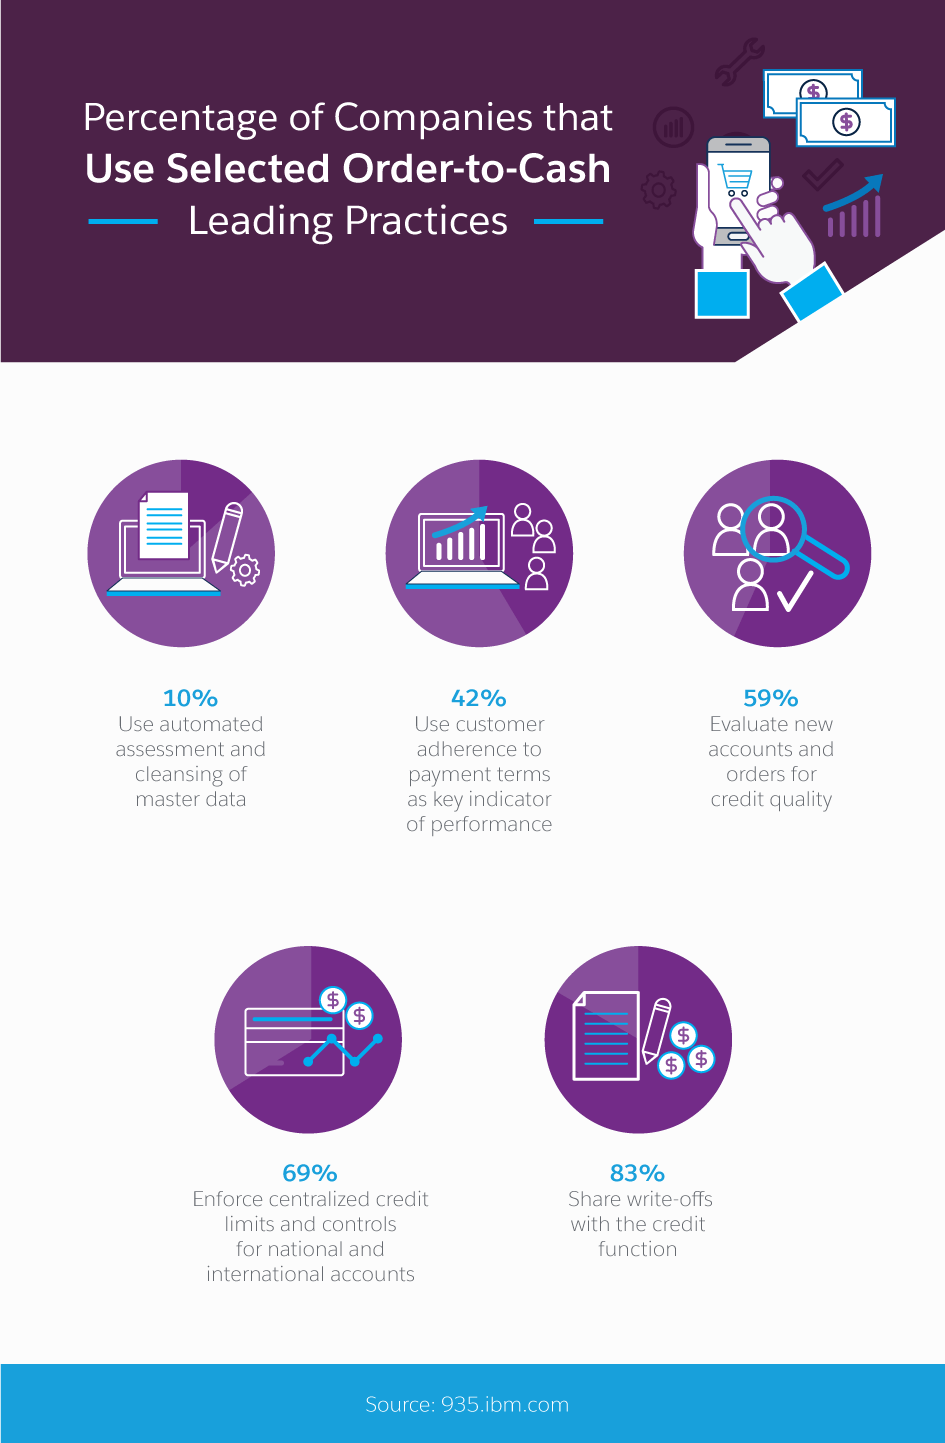
\includegraphics[width=10cm]{wong.png}
	\caption{Het aantal bedrijven dat gebruik maakt van een order-to-cash proces. \textcite{Wong2018}}
	\centering
\end{figure}
  
Bij een OTC is technologie cruciaal. Elk deeltje van het proces kan beter worden door een correcte implementatie van microservices. Die kunnen ervoor zorgen dat de automatisering vlotter verloopt.

In figuur 2.18 wordt dit afgebeeld in een schema.
\begin{figure}[h!]
	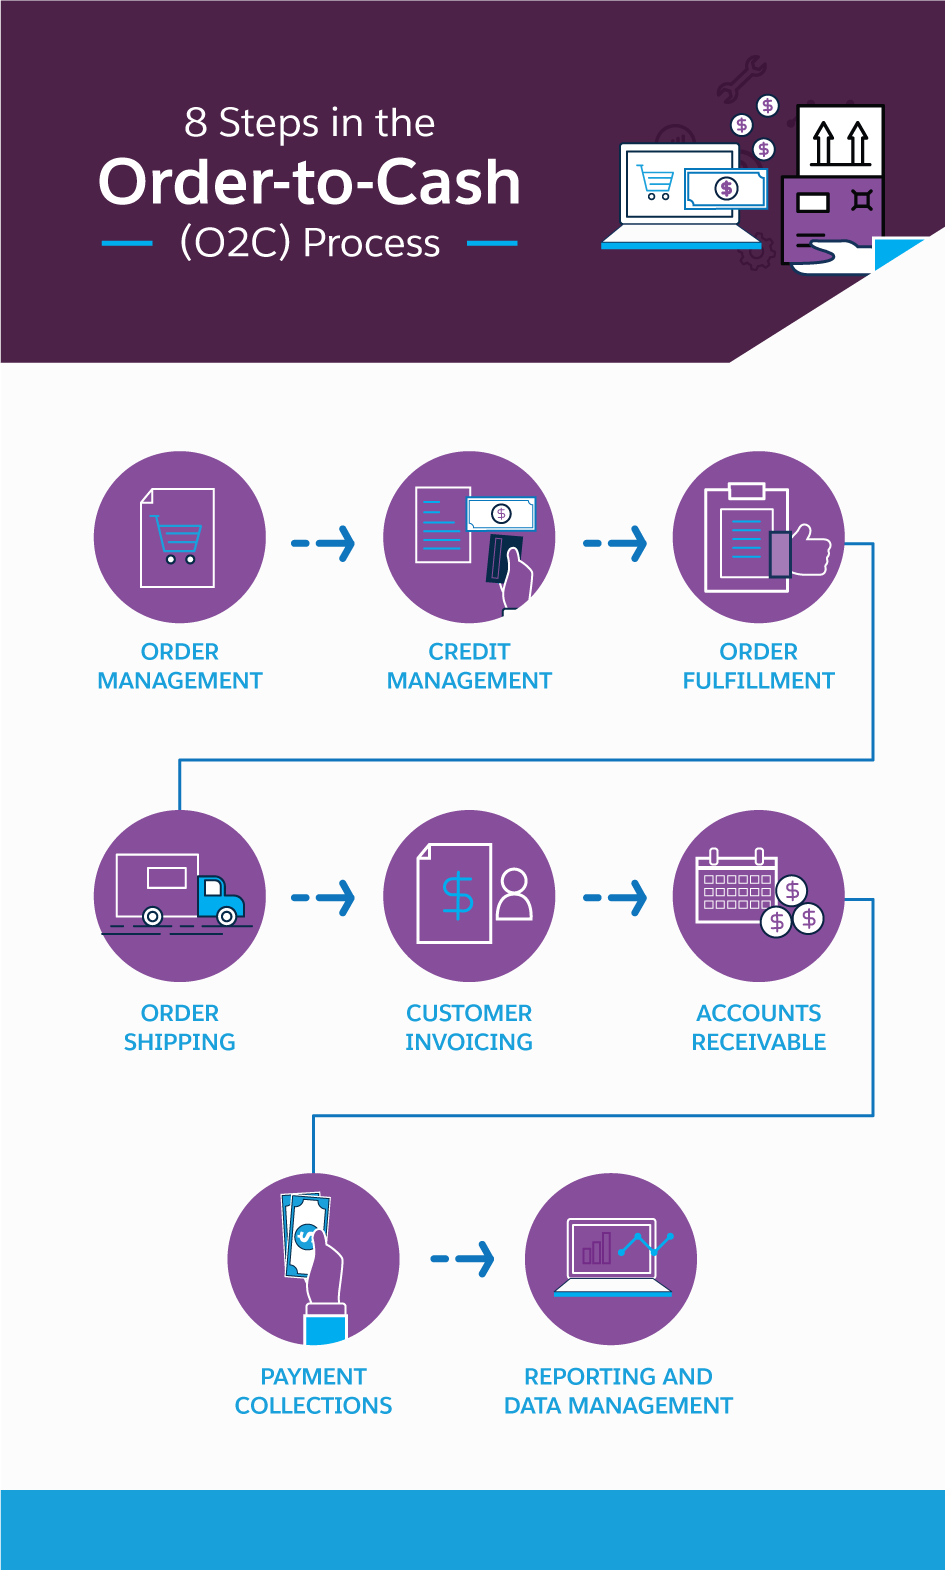
\includegraphics[width=10cm]{wong2.png}
	\caption{Het order-to-cash proces. \textcite{Wong2018}}
	\centering
\end{figure}


\subsection{Technologie: Wat biedt SAP zelf aan voor microservices}
SAP biedt een open-source project aan genaamd Kyma om microservices te implementeren.
Kyma maakt de werking met microserivces eenvoudiger. Kubernetes wordt gebruikt om applicaties op verschillende machines te managen. Het kan onder meer gebruikt worden om cloud-based en on-premise applicaties om te zetten naar een microservice architectuur. Cloud-based applicaties zijn applicaties die hun data gaan ophalen op het internet in plaats van op de harde schijf van de computer. On-premise is lokaal op de computer, op de harde schijf. Kyma zorgt voor betere end-to-end ervaring voor scenario's, \textcite{Kyma2019}.

Binnen SAP wordt er omgegaan met software van verschillende leveranciers. SAP probeert om hun software te customizen naar de  wensen van de klant. Dit vraagt meer openheid en een modernere architectuur. 
Het idee achter Kyma is het creëeren van serverless applicaties, mashups en microservices. Het kan  gebruikt worden om snel kleine, gecustomizede modules te ontwikkelen. 

Knative is een platform dat developers ondersteunt om serverless applicaties te maken op Kubernetes en dat samenwerkt met Kyma. Dit zorgde voor groot enthousiasme bij SAP omdat hun Kyma project een bevestiging kreeg. Al snel  werd Kyma gerefactored om samen te kunnen  werken met Knative. Er werden overlappende componenten  weggelaten, wat Kyma slanker en gestroomlijnder maakt. Dankzij Knative kan Kyma zich richten op higer-level enterprise applications en service consumption scenario's, \textcite{Semerdzhiev2018}.

De samenwerking tussen Kyma en Knative is belangrijk. Er wordt een complete set van bouwblokken aangeboden en het zijn twee sterke frameworks. Bij het gebruik van beide kunnen er could-native oplossingen gebouwd worden op Kubernetes met een sterk framework. Op figuur 2.19 is te zien wat Kyma en Knative aanbiedt. \textcite{Hofmann2018}
\begin{figure}[h!]
	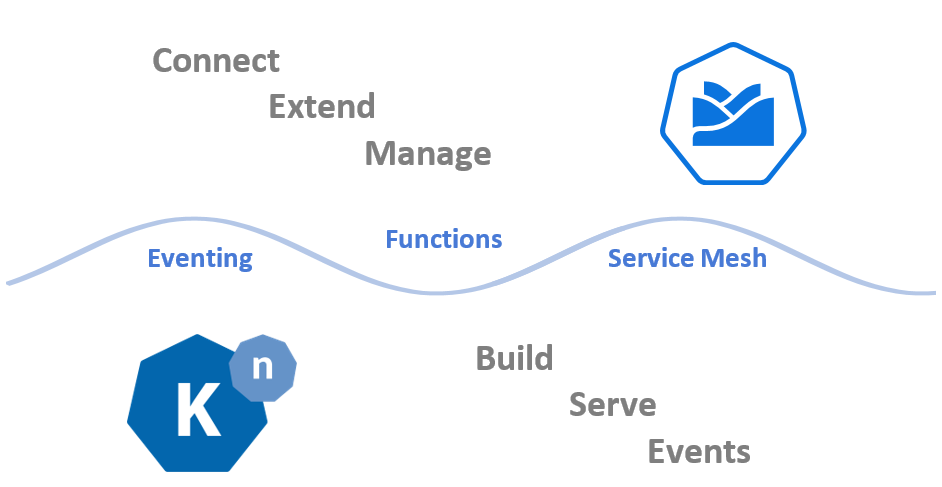
\includegraphics[width=10cm]{1-kyma-knative.png}
	\caption{Wat Kyma, boven de lijn, aanbiedt en wat Knative, onder de lijn, aanbiedt \textcite{Hofmann2018}.}
	\centering
\end{figure}


\section{Requirements van de business}
Het OTC proces heeft het volgende nodig van een bedrijf, \textcite{Biedron2018}
\begin{itemize}
	\item De klant moet een order of meerdere orders kunnen plaatsen. Een goed werkend order-systeem is een must.
	\item Het order ophalen uit de voorraad. Er moet een goed voorraadbeheer aanwezig zijn. Dit moet ervoor zorgen dat het aantal laattijdige leveringen geminimaliseerd wordt. Samen met een goed voorraadbeheer wordt ook best bijgehouden waar men goederen geplaatst heeft in het magazijn.
	\item De levering moet goed gepland worden. Dit zou voor het grootste deel al geautomatiseerd moeten zijn. Een email met informatie over de levering is hierbij een verplichting. 
	\item Het aanmaken van een factuur op basis van het geplaatst order met de juiste klantgegevens moet een geautomatiseerd onderdeel worden. 
	\item De betaling van de factuur komt toe in de financiele afdeling. Automatische afhandeling is een verplichting.
\end{itemize}
Bij een order plaatsen, komen de volgende elementen aanbod:
\begin{itemize}
	\item Er moet een lijst met producten beschikbaar zijn.
	\item De klant zijn gegevens moeten gekend zijn bij het bedrijf.
	\item Het systeem bij het bedrijf moet beschikbaar zijn.
\end{itemize}
Na het plaatsen van het order dat klaargezet worden om te leveren, zijn volgende elementen van belang:
\begin{itemize}
	\item Een goed voorraadbeheer is de eerste must.
	\item Een overzicht van waar alles staat, geeft een meerwaarde.
	\item Bij het ophalen van een product om bij een order te plaatsen, moet de hoeveelheid in de voorraad verminderen.
\end{itemize}

%%=============================================================================
%% Methodologie
%%=============================================================================

\chapter{\IfLanguageName{dutch}{Methodologie}{Methodology}}
\label{ch:methodologie}

In dit hoofdstuk zal er een schets gemaakt worden van het OTC proces met een microservice architectuur. De architectuur zal aangepast worden aan de hand van integratie patterns aangehaald in 'Stand van zaken'. 

Als eerste werd de volledige architectuur uit elkaar gehaald. Zoals het eerste anti-pattern: break the piggy break. Maar één van de veel voorkomende fouten bij het anti-pattern is de databank. Om ervoor te zorgen dat de databank niet dezelfde blijft als die uit de monolithic architectuur, wordt er data integratie toegepast. Eens de microservices en de databank uitgedacht zijn, moet de communicatie uitgedacht worden. De theoretische uitleg van de communicatiemethode is terug te vinden. De communicatiemethode zal toegepast worden op de architectuur die verworven wordt uit de bovenstaand vernoemde integratie patterns.
Eens elk onderdeel aangebracht is, wordt alles samengebracht tot de complete architectuur.

\section{Anti-pattern: Break the piggy bank}
Zoals beschreven in het onderdeel 'Stand van zaken' wordt de gehele applicatie in stukjes opgedeeld. Er wordt gekeken naar de business functionaliteiten. 
In de volgende sectie worden de verschillende microservices besproken. Elke stap van het order-to-cash proces is een microservices. Maar de stappen bevatten meerdere business functionaliteiten. Het zou tegen de principes van microservices zijn. Per stap van het proces werd gekeken naar de functionaliteiten. Eens die gedefineerd waren, werd er gekeken naar de gelijke funcitonaliteiten over de verschillende stappen heen. Die functionaliteiten werden in microservices opgedeeld. Elke stap van het order-to-cash proces spreekt de microservices aan die van belang zijn. Een belangrijk punt: de databank bij deze manier van werken blijft dezelfde als monolithic. De databank wordt verder behandelt in het gedeelte 'Data Integratie'.

Er werd gekozen om de microservice niet nog kleiner te maken om het overzichtelijk te houden. Nu weet men welke microservice men moet gebruiken wanneer er iets met orders moet gebeuren.   

Een microservice is schaalbaar. Omdat de volgende requirement meermaals voorkomen in het proces, is het voordeliger om te dupliceren en te hergebruiken van deze microservices.


\subsubsection{Klantengegevens ophalen}
Veel onderdelen van het OTC proces moeten de klantgegevens kunnen raadplegen. Om te zorgen dat alles op een gelijke manier gebeurt, is hier een microservice van gemaakt.
Deze microservice gaat ervoor zorgen dat de klantengegevens uit de databank worden gehaald.
Deze microservice komt voor in volgende onderdelen van het OTC proces:
\begin{itemize}
	\item Order management
	\item Credit management
	\item Order shipment
	\item Klant management
	\item Facturatie
	\item Accounts receivables
\end{itemize}

\subsubsection{Orders plaatsen, ophalen en verwijderen}
Een belangrijk onderdeel is het plaatsen, ophalen en verwijderen van orders. Er zijn een aantal onderdelen van het OTC proces die de specificaties van een order moeten weten. Zo is het voor de facturatie en het opstellen van de levernota's belangrijk.
Dit microservice wordt gebruikt in volgende onderdelen:
\begin{itemize}
	\item Order management
	\item Credit management
	\item Order fullfilment
	\item Order shipment
	\item Facturatie
	\item Klant management
\end{itemize}

\subsubsection{Producten ophalen en het aantal in voorraad veranderen}
In het order-to-cash proces worden er geen producten toegevoegd aan de lijst, dus moet dit niet in een microservice gestoken worden. De stuks op voorraad moet aangepast wanneer er een product uit de rekken wordt gehaald en bij een bestelling wordt geplaatst. Bij het ophalen van een product wordt de verkoopprijs opgehaald en toegevoegd aan de orderlijn.
De microservice zal gebruikt worden in volgende onderdelen:
\begin{itemize}
	\item Order management
	\item order fullfilment
\end{itemize}

\subsubsection{Facturatie maken en ophalen}
Eén van de laatste stappen in het order-to-cash proces. Facturen maken en ophalen zijn van groot belang bij een order-to-cash proces.De producten op de factuur moeten overeenstemmen met wat geleverd werd. Het is van groot belang dat achteraf kan gekeken worden of de factuur klopt met de order. De factuur wordt opgesteld aan de hand van het order. 
Deze microservice komt voor in het onderdeel facturatie.

\subsubsection{Shipment documentatie opstellen}
Het shipment document wordt gegenereerd op basis van het order. Er wordt gekeken naar het ordernummer en dan wordt er gekeken naar het klantnummer. Hierna wordt dan de microservice om klantgegevens op te halen aangesproken om de gegevens van de specifieke klant op te halen. Dit microservice wordt enkel gebruikt binnen het onderdeel verzending.

\subsubsection{Aanmaning opmaken en verwijderen}
Het opmaken en verwijderen van aanmaningen gebeurt enkel als er sprake is van achterstallige betaling. Dit zou niet vaak mogen voorkomen. 

\subsubsection{Berichten plaatsen op de queue}
Berichten plaatsen op de queue omvat dat de gegevens die de volgende stap in het OTC proces nodig heeft, correct op de wachtrij van de volgende stap geplaatst wordt.  Het is dan eenvoudiger om er een microservice van te maken, zodat elk onderdeel op een uniforme manier het bericht plaatst. 
Deze microservice komt voor in elk onderdeel van het proces.

\subsubsection{Berichten ophalen van de queue} 
Elk onderdeel moet berichten van zijn queue kunnen halen. Aangezien dit vaak voorkomt wordt er een microservice van gemaakt om te zorgen dat dit opeen vlotte en uniforme manier gebeurt. 
Deze microservice komt voor in elk onderdeel van het proces.

\section{Data integration}
Bij 'break the piggy bank' wordt de databank behouden van de vorige architectuur. Dat leidt meestal tot de doodsteek van de microservices architectuur. De databank niet aanpassen, kan leiden tot falen op langere termijn. Daarom is data integratie een correcte manier om de databank aan te passen naar één die de microservices architectuur wel aan kan.

Elke microservice heeft zijn databank. De microservices betreffende de stappen van het order-to-cash proces hebben geen databank. Zij geven enkel commando's door aan de microservices die een business requirement als functionaliteit hebben. De microservices met de business requirement hebben elk hun eigen databank. Elke microservices omvat een eigen domein. Hierdoor zal er nergens gedupliceerde data terug te vinden zijn. Op figuur 3.1 is te zien hoe de databank structuur eruit ziet. De lijnen tussen de databank geeft weer welke verbindingen er liggen. 
\begin{figure}[h!]
	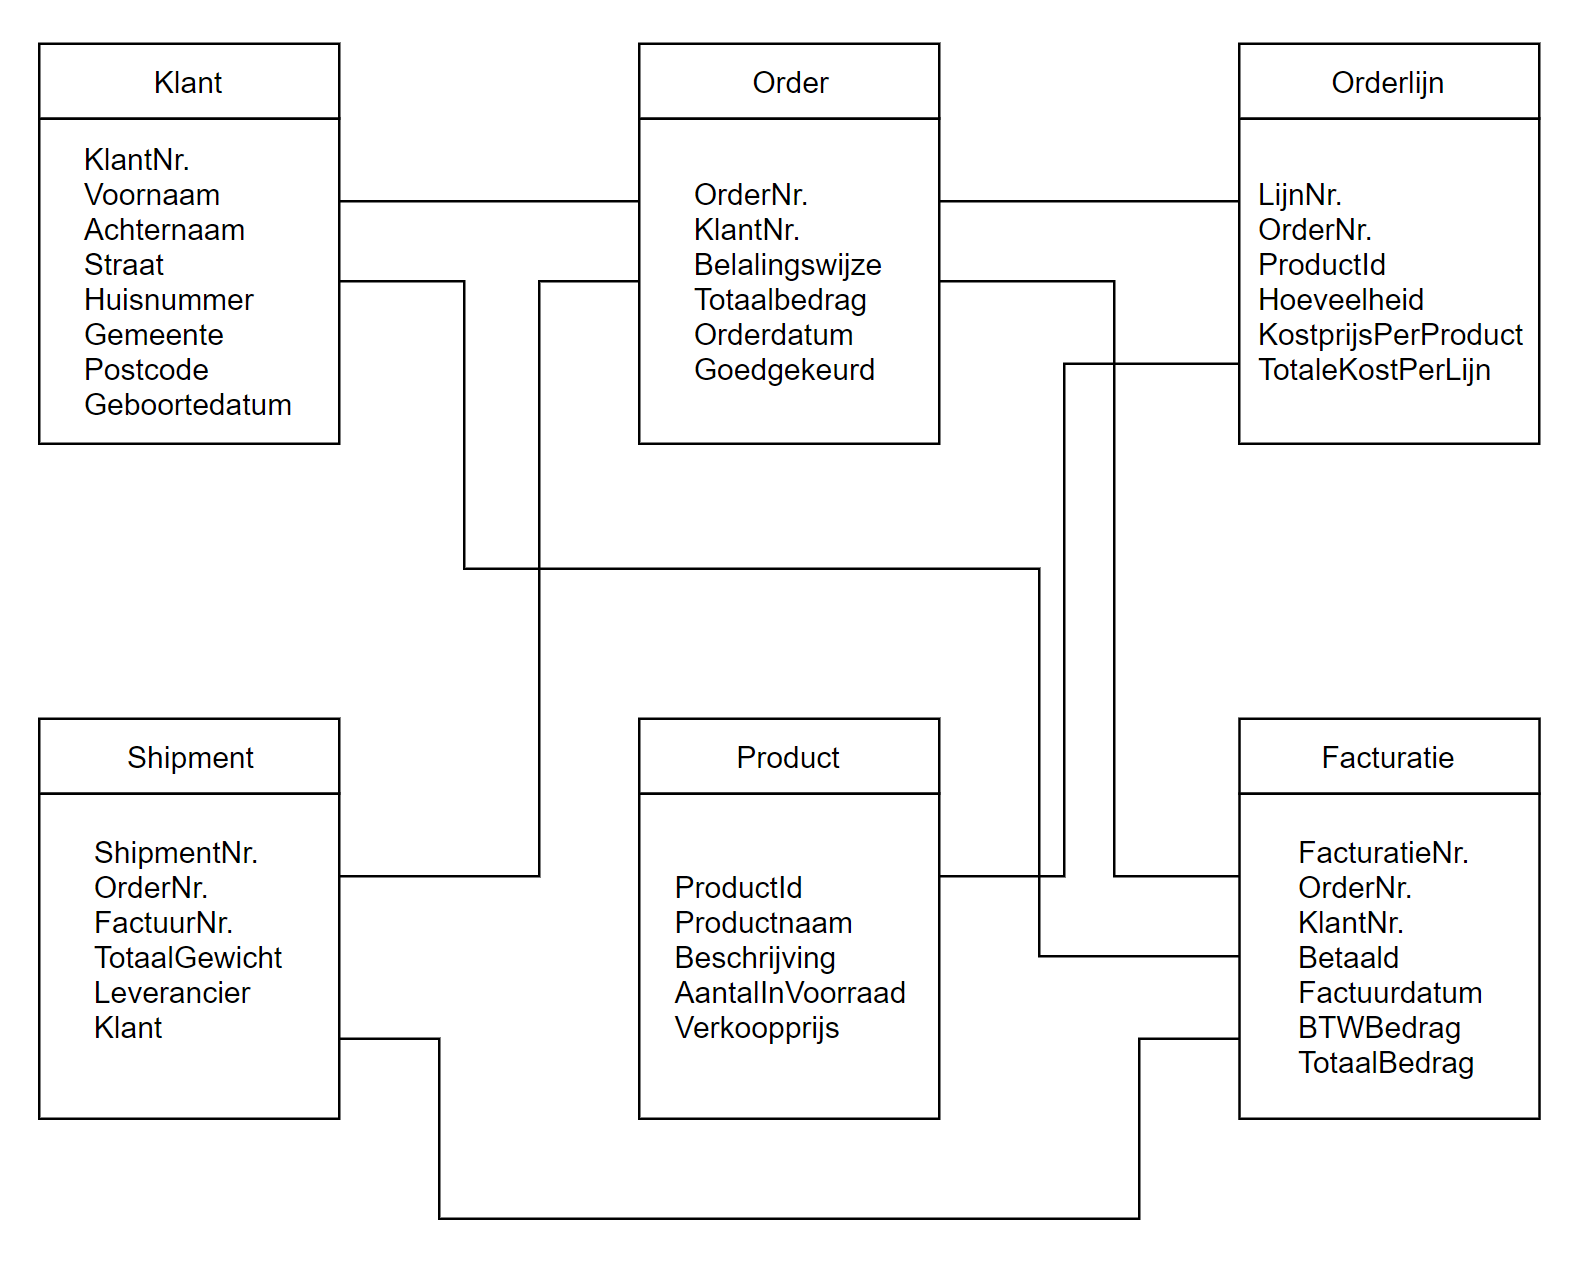
\includegraphics[width=15cm]{databank.png}
	\caption{De databank structuur.}
	\centering
\end{figure}

Een order heeft een klantnummer om te weten welke klant het order plaatste. Credit management kan de eigenschap bij het order veranderen van 'goedgekeurd' naar 'niet goedgekeurd'. Van ieder order wordt een orderlijn bijgehouden waraan een product of services is verbonden. Naast het product is ook een beschrijven en verkoopprijs te vinden. Het aantal in voorraad is gekend omdat bij het order fullfilment moet de voorraad aangepast worden van het specifieke product. Omdat een factuur gebaseerd is op een order, is het zo de klant gekend en zo klopt de factuur met de order. De klantengegevens moeten gekend zijn om naar het juiste adres te factureren.

Elke databank heeft een queue. Wanneer een microserivce B iets nodig heeft van microserivce A, kan die vraag naar de queue gepost worden.

De databank van microservice 'klant gegevens ophalen' zal alle data van de klanten bevatten.
De databank van microservice 'order plaatsen, ophalen en verwijderen' zal alle data van de orders bevatten.
De databank van microservice 'producten ophalen en aantal in de voorraad veranderen' zal alle data van de producten bevatten.
De databank van microservice 'facturatie maken en ophalen' alle data van de facturatie bevatten.
De databank van microservice 'Shipment documentatie opstellen' bevat de data van de orders om aan de hand van die data, de documenten op te stellen en dan toe te voegen aan de data met alle shipment documenten.
De databank van microservice 'Aanmaning opmaken en verwijderen' bevat alle data van de aanmaningen. 
De microservices 'bericht op queue plaatsen' en 'bericht van de queue halen', hebben geen datastore. Het zijn twee microservices die geen data moeten gaan ophalen of wegschrijven. Ze staan in voor het ophalen en plaatsen van berichten. 

\section{Communicatie tussen de microservices}
De communicatie gebeurt aan de hand van messaging. Maar omdat het order-to-cash een proces is waarin alleen voorwaarts kan worden gegaan. Daardoor is hier geen nood aan een message broker. Maar er wordt wel gewerkt met een queue. Omdat deze als voordeel heeft dat de microservices niet overbelast geraakt. De microservices handelt alles op zijn tempo. 
Klant 66 plaatst een order met vier verschillende producten. Het ordernummer is 23. De volledige bestelling komt binnen in het systeem en wordt op de queue van ordermanagement geplaatst. Het order wordt van de queue gehaald aan de hand van consumption en acknowledgement. Ordermanagement verwerkt de binnengekomen order. Dan wordt het klantnummer en ordernummer op de queue van creditmanagement geplaatst. Creditmanagement haalt het bericht van de queue en kijkt naar het betaalgedrag van de klant. Staat de klant gekend voor wanbetalen, dan wordt er geen goedkeuring gegeven om het order te plaatsen. Bij een corect betaalgedrag, krijgt het order goedkeuring om geplaatst te worden. Dan wordt het ordernummer doorgestuurd naar het volgende deel van het proces. 
Dus volgende queue's zouden moeten bestaan:
\begin{itemize}
	\item QorderMan is een queue voor order management.
	\item QcreditMan is een queue voor credit management.
	\item QorderFul is een queue voor order fulfilment.
	\item QorderShip is een queue voor order shipment.
	\item Qfact is een queue voor de facturatie.
	\item QaccountsRec is een queue voor accounts receivable. 
\end{itemize}

Niet alle data wordt volledig naar de queue gestuurd. Enkel belangrijke data zoals het klantennummer wordt verstuurd naar creditmanagement. Daar wordt dan aan de hand van het klantnummer de bestelgegevens opgehaald en nagegaan of die klant wel een order mag plaatsen. Het ordernummer wordt meegestuurd om zeker te zijn dat het correcte order goed- of afgekeurd wordt. Zo blijft de overhead op de queue minimaal. Om meer gegevens op te halen, moet de databank aangesproken worden. De gehele structuur van de databank wordt beschreven in het volgende gedeelte.

\subsection{De communicatie tussen de onderdelen van het OTC proces}

\begin{figure}[h!]
	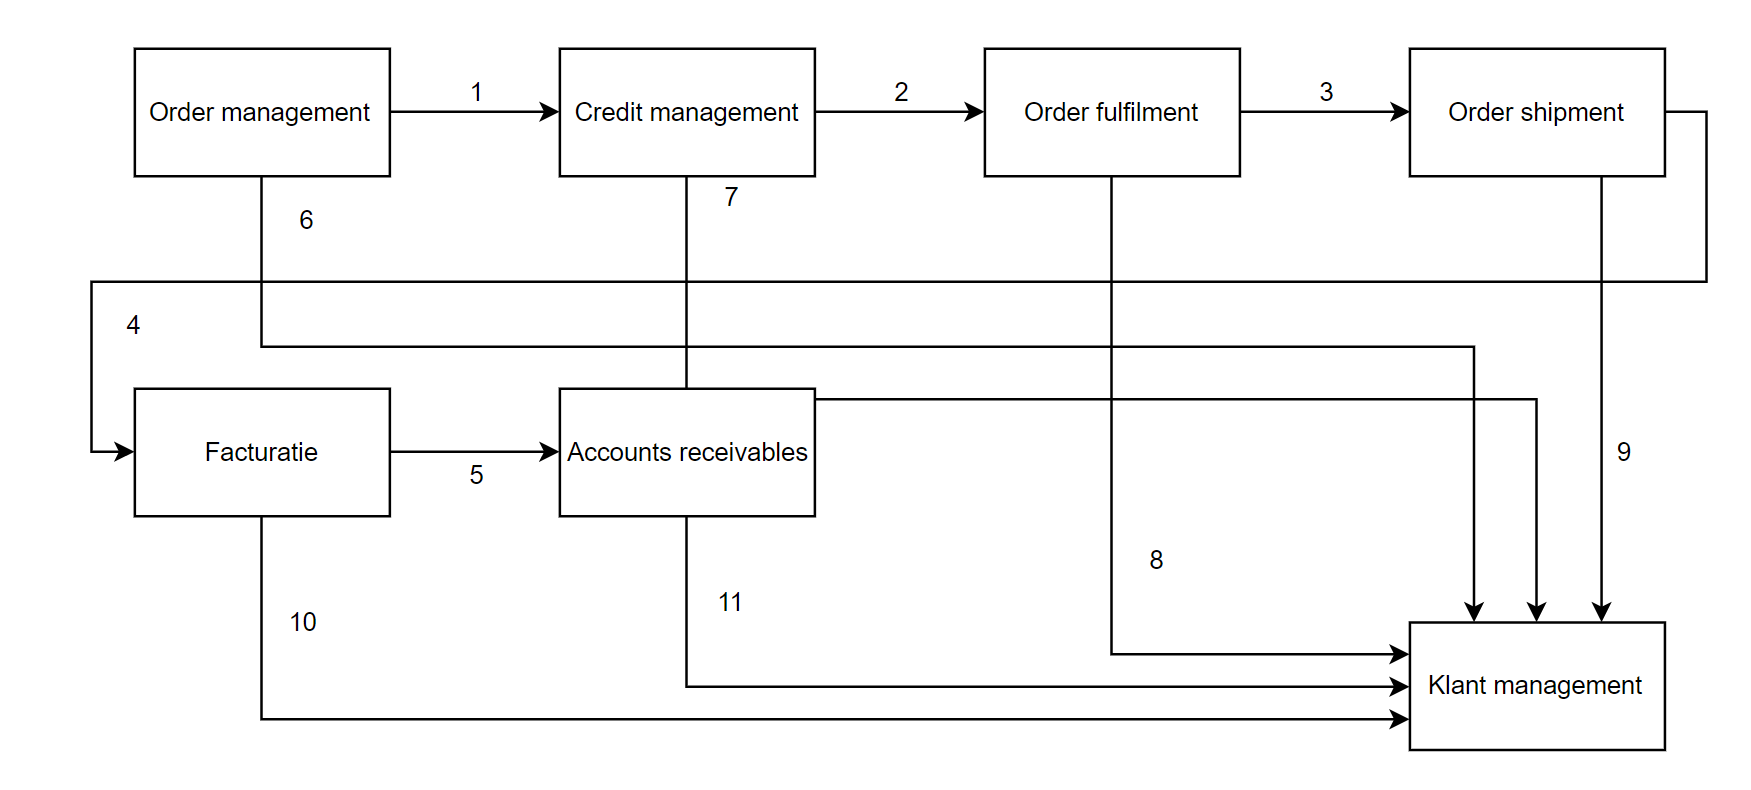
\includegraphics[width=15cm]{schema_communicatie.png}
	\caption{De communicatie tussen de verschillende onderdelen van het order-to-cash proces.}
	\centering
\end{figure}
Zoals eerder vermeld, is elk onderdeel van het OTC proces een microservice. Elk onderdeel spreekt kleinere microservices aan die de verschillende requirements van elke stap uitvoeren.
Op figuur 3.2 is het communicatie patroon zichtbaar.
Voordat het proces van start kan gaan, moet een klant een order plaatsen. Een order bevat een aantal producten. Eens de klant een order geplaatst heeft dan is er een ordernummer aangemaakt. Belangrijk hierbij is ook dat er telkens een ordernummer verzonden wordt aan een onderdeel.
Meer uitleg over wat elk onderdeel doet, bevindt zich in het volgende hoofdstuk.
De nummers van de opsomming komen overeen met die op afbeelding 3.2.
\begin{enumerate}
	\item De communicatie tussen ordermanagement en creditmanagement. Er is een order geplaatst door klant 66. Ordermanagement zorgt ervoor dat het order in de databank geraakt. Eens de taak van ordermanagement is gedaan, plaatst die het klantnummmer en het ordernummer op de queue van creditmanagement. 
	\item De communicatie tussen creditmanagement en order fullfilment. Creditmanagement heeft het ordernummer en klantnummer van ordermanagement gekregen. Het bericht wordt van de queue gehaald. Creditmanagement gaat dan aan de hand van de klantgegevens beslissen of de klant het order mag plaatsen of niet. Is het order goedgekeurd, dan wordt het ordernummer op de queue van order fullfilment gezet.
	\item De communicatie tussen order fullfilment en order shipment. Order fullfilment heeft het ordernummer doorgekregen van credit management. Dit geeft het ordernummer door aan order shipment eens zijn taak gedaan is. 
	\item De communicatie tussen order shipment en de facturatie. Het ordernummer werd op de queue van order shipment geplaatst. Eens alles opgemaakt is bij order shipment, wordt het ordernummer doorgestuurd naar de facturatie.
	\item De communicatie tussen facturatie en accounts receivables. De facturatie kreeg een bericht van order shipment om de factuur op te maken voor het order met des betreffende ordernummer. Is de taak van facturatie afgerond, dan wordt het factuurnummer doorgestuurd naar accounts receivables. Op die manier de betaling verder opgevolgd worden.
	\item Ordermanagement plaatst het ordernummer op de queue van klant management. Klant management stuurt een bevestiging naar de klant van het order en laat weten dat er eerst een controle komt op het betaalbedrag van de klant.
	\item Creditmanagement plaatst het ordernummer en de status van goedgekeurd of afgekeurd op de queue. Deze status wordt in een bericht naar de klant verzonden. 
	\item Order fullfilment plaatst een bericht op de queue om te laten weten de goederen uit het magazijn werden opgehaald en klaar staan voor verzending.
	\item Order shipment plaatst een bericht op de queue wanneer de goederen klaar zijn voor vertrek. Klant management zorgt er dan voor dat het bericht tot bij de klant geraakt.
	\item Facturatie plaatst een bericht op de queue van klant management om ervoor te zorgen dat de factuur tot bij de klant geraakt.
	\item Accounts receivables plaatst een bericht op de queue van klant management als er aanmaningen moeten worden gestuurd.
\end{enumerate}

\subsection{De architectuur}
In volgende tabel zijn letters en bijhorende microservices terug te vinden. Deze worden gebruikt bij het uitleggen van de architectuur.
\begin{table}[]
	\resizebox{\textwidth}{!}{%
		\begin{tabular}{|l|p{15cm}|}
			\hline 
			A & Klantgegevens ophalen \\ \hline
			B & Orders plaatsen, ophalen en verwijderen \\ \hline
			C & Producten ophalen en het aantal op voorraad aanpassen \\ \hline
			D & Shipment documenten opstellen \\ \hline
			E & Facturatie maken en ophalen \\ \hline
			F & Aanmaning opmaken en verwijderen \\ \hline
			G & Bericht plaatsen op de queue \\ \hline
			H & Bericht ophalen uit de queue \\ \hline
		\end{tabular}%
	}
	\caption{Legende die gebruikt wordt in de afbeeldingen.}
\end{table}

In tabel 3.1 is de legende terug te vinden die gebruikt wordt bij het uitleggen van elk onderdeel apart.
In figuur 3.3 is te zien hoe het volledige proces communiceert met de verschillende microservices. Elk onderdeel van het proces is een microservice op zich.
\begin{figure}[h!]
	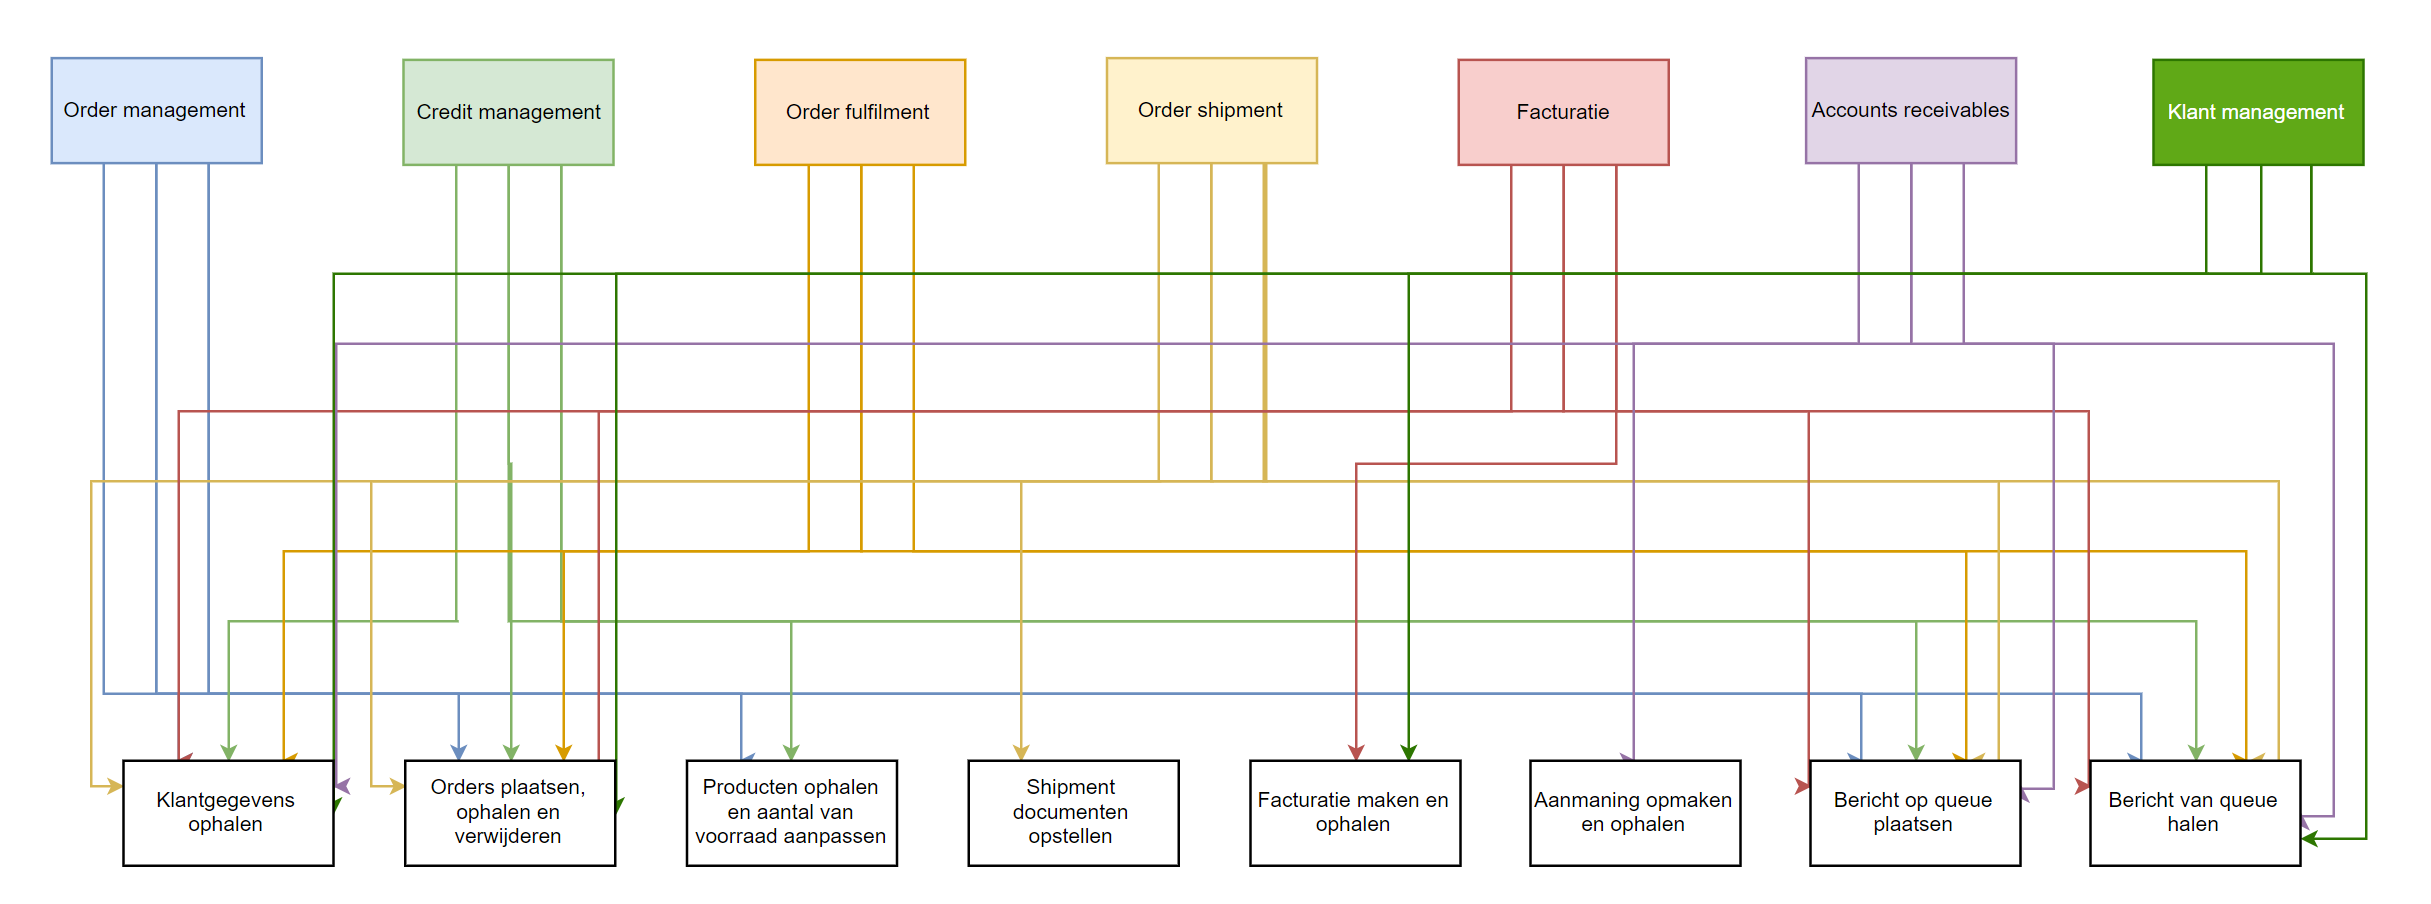
\includegraphics[width=15cm]{schema_microservices.png}
	\caption{Welk onderdeel, welke microservices aanspreekt.}
	\centering
\end{figure}

\subsubsection{Order management}
\begin{figure}[h!]
	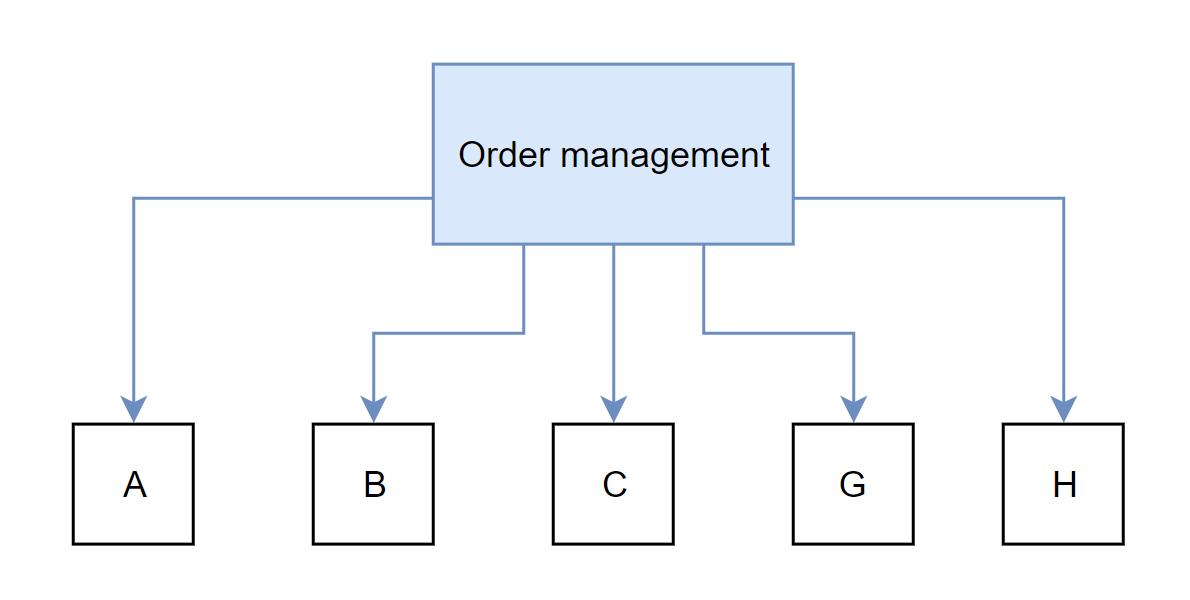
\includegraphics[width=5cm]{ordermanagement.png}
	\caption{Order management communiceert met volgende microservices.}
	\centering
\end{figure}
Order management communiceert met volgende microservices:
\begin{itemize}
	\item Klantengegevens ophalen.
	\item Orders plaatsen, ophalen en verwijderen.
	\item Producten ophalen en het aantal van de voorraad aanpassen.
	\item Bericht plaatsen op queue.
	\item Bericht van queue halen.
\end{itemize}
Een klant plaatst een order op het platform van het bedrijf. De gegevens van de klant worden opgehaald en gelinkt aan het nieuw gecreëerde order. Eens die twee taken zijn afgerond, wordt het bericht op de queue geplaatst van credit management.

\subsubsection{Credit management}
\begin{figure}[h!]
	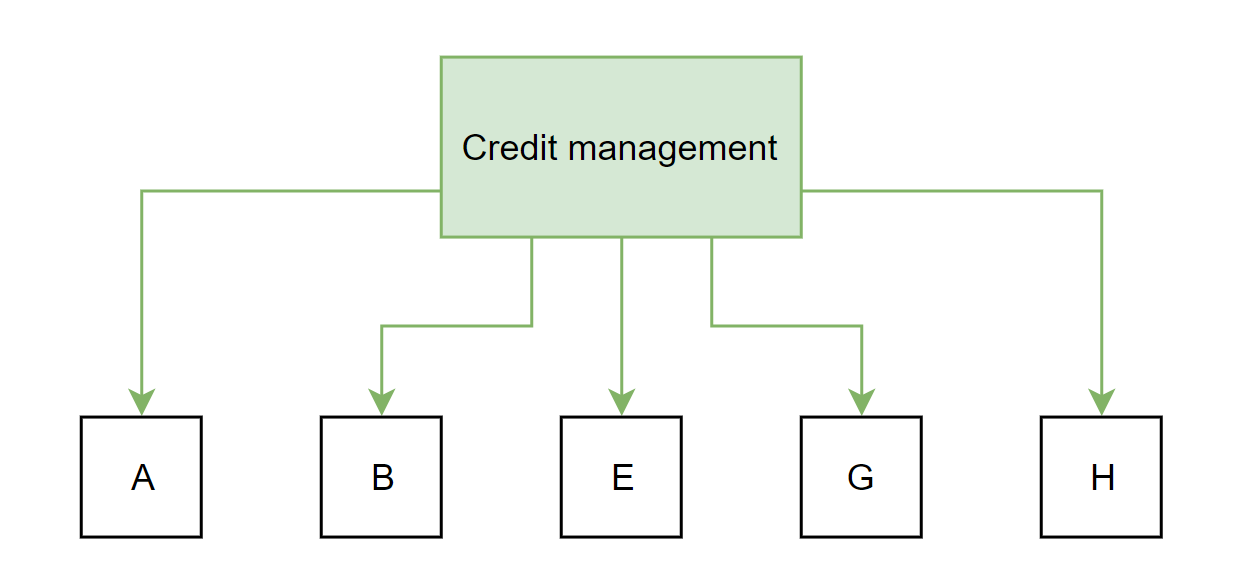
\includegraphics[width=5cm]{creditmanagement.png}
	\caption{Credit management communiceert met volgende microservices.}
	\centering
\end{figure}
Credit management communiceert met volgende microservices:
\begin{itemize}
	\item Klantengegevens ophalen.
	\item Orders ophalen, plaatsen en verwijderen.
	\item Facturatie maken en ophalen.
	\item Bericht plaatsen op queue.
	\item Bericht van queue halen.
\end{itemize}
Eerst wordt het bericht opgehaald dat order management op de queue plaatste, opgehaald. Daarna wordt er een klantennummer en ordernummer verzonden. Credit management kijkt of de klant een goed betaalgedrag heeft. Is de klant bekend als wanbetaler dan wordt het order afgekeurd. In andere gevallen krijgt het order een goedkeuring en wordt het ordernummer geplaatst op de queue van order fullfilment. Dan zit de taak van credit management erop.

\subsubsection{Order fullfilment}
\begin{figure}[h!]
	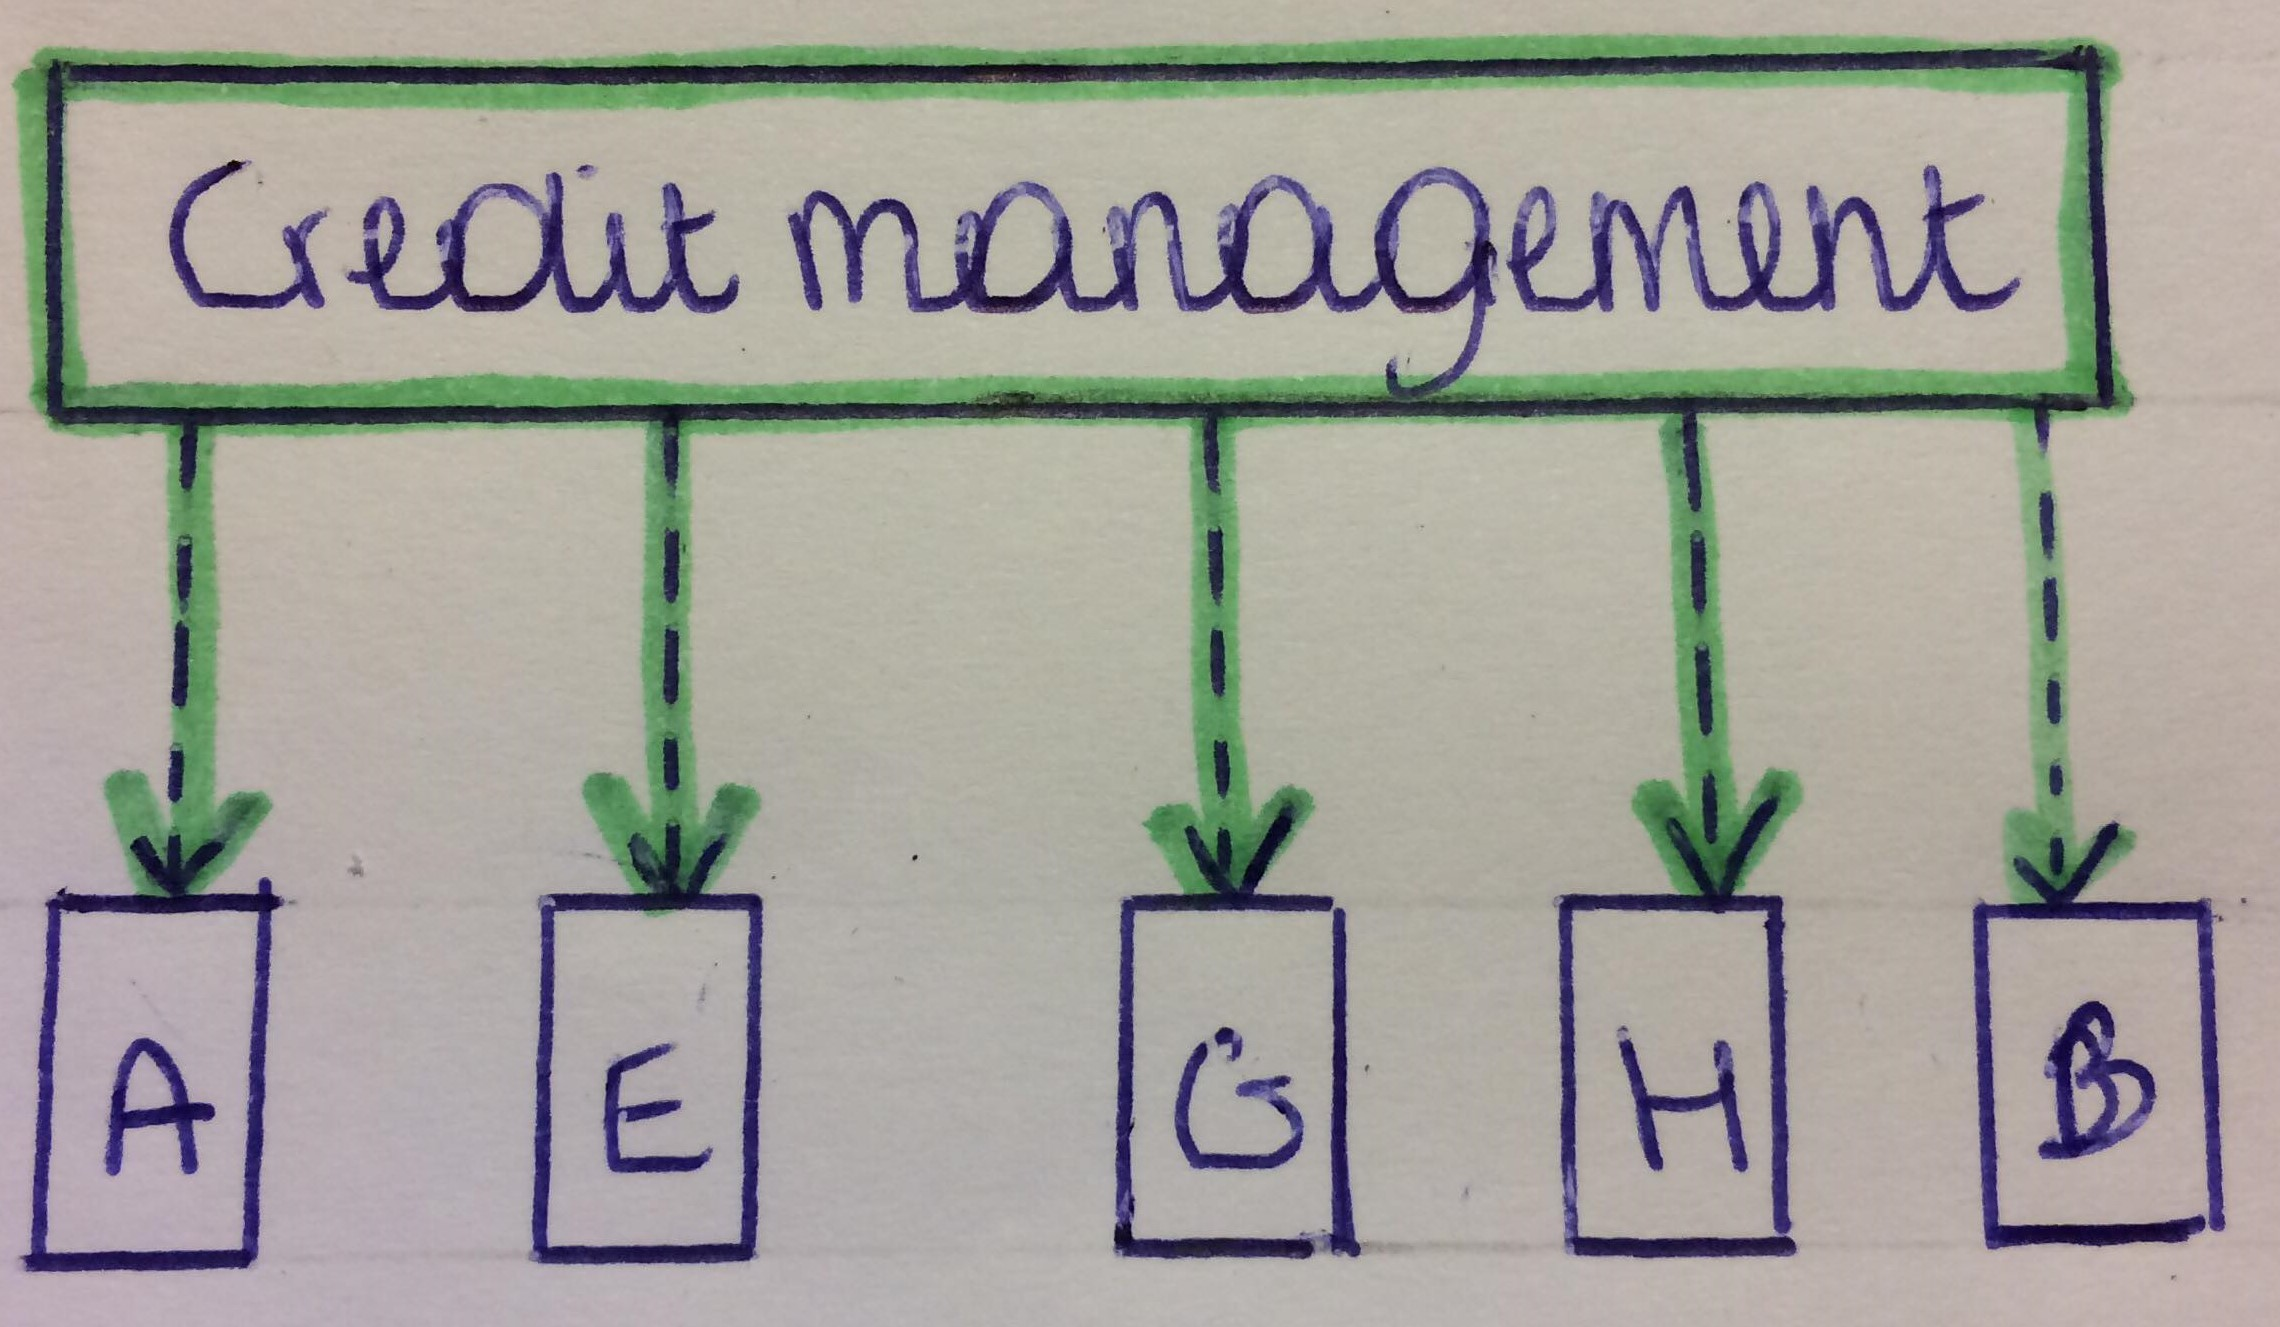
\includegraphics[width=5cm]{orderfullfilment.png}
	\caption{Order fullfilment communiceert met volgende microservices.}
	\centering
\end{figure}
Order fullfilment communiceert met volgende microservices:
\begin{itemize}
	\item Orders ophalen, plaatsen en verwijderen.
	\item Producten ophalen en het aantal in de voorraad aanpassen.
	\item Bericht plaatsen op queue.
	\item Bericht van queue halen.
\end{itemize}
Bij order fullfilment staat een ordernummer op de queue. Dit wordt opgehaald en geef aan welke goederen er uit het magazijn moeten gehaald worden. Voor alle goederen moet het aantal in de voorraad aangepast worden. Eens het order compleet is, wordt het ordernummer op de queue van order shipment geplaatst.

\subsubsection{Order shipment}
\begin{figure}[h!]
	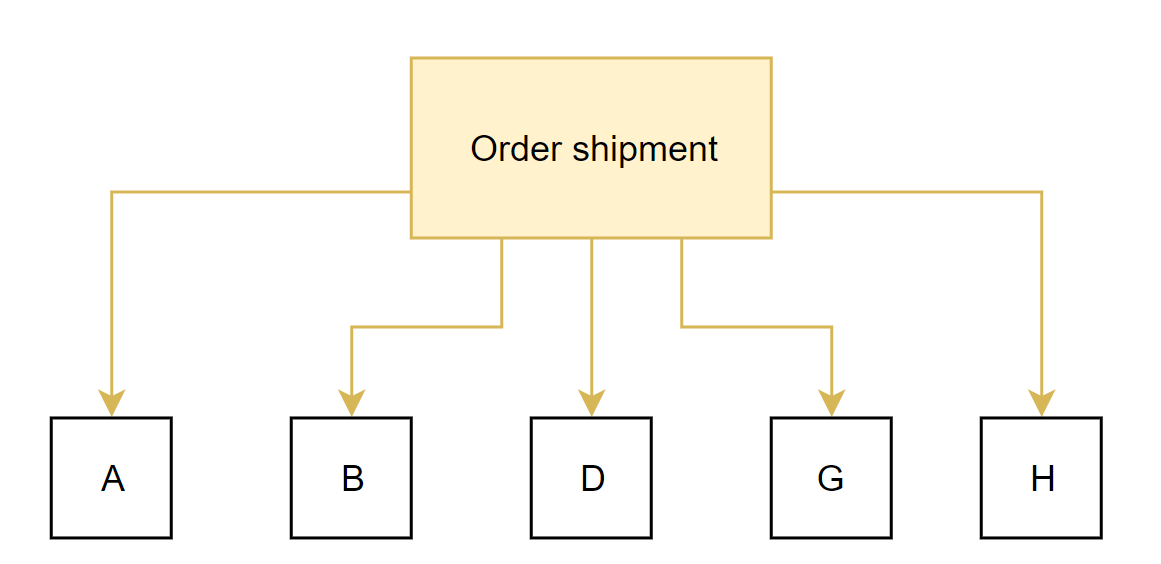
\includegraphics[width=5cm]{ordershipment.png}
	\caption{Order shipment communiceert met volgende microservices.}
	\centering
\end{figure}
Order shipment communiceert met volgende microservices:
\begin{itemize}
	\item Orders ophalen, plaatsen en verwijderen.
	\item Klantengegevens ophalen.
	\item Shipment document opstellen.
	\item Bericht plaatsen op queue.
	\item Bericht van queue halen.
\end{itemize}
Order shipment krijgt het ordernummer binnen via zijn queue. Het order wordt bekeken en de klantengegevens worden opgehaald aan de hand van het klantnummer dat gekoppeld werd aan het order. Eens het order shipment document is opgesteld en alle goederen klaar zijn voor vertrek, wordt het ordernummer geplaatst op de queue van facturatie.

\subsubsection{Facturatie}
\begin{figure}[h!]
	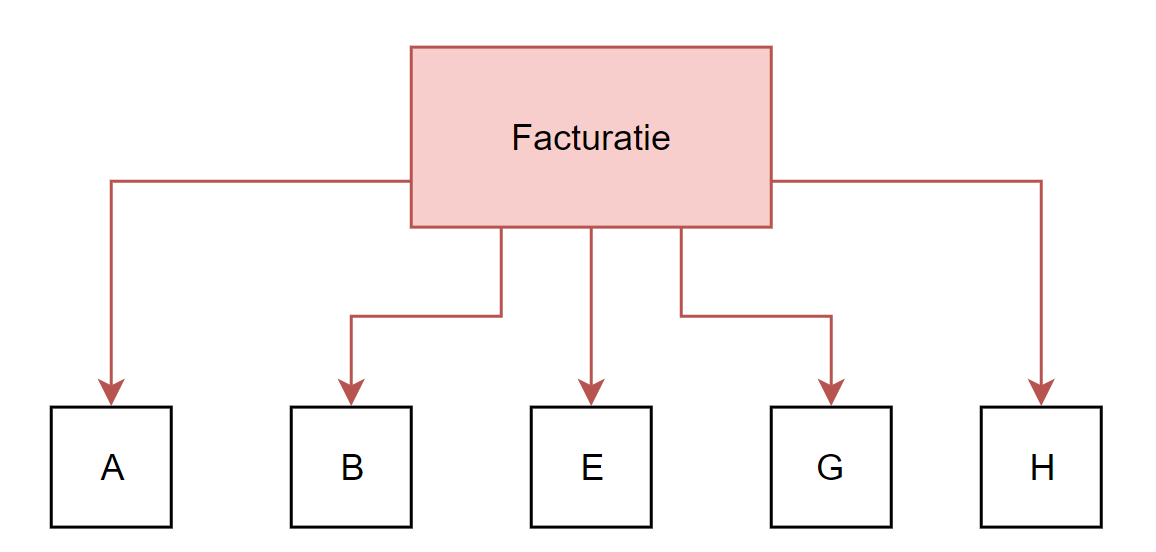
\includegraphics[width=5cm]{facturatie.png}
	\caption{Facturatie communiceert met volgende microservices.}
	\centering
\end{figure}
Facturatie communiceert met volgende microservices:
\begin{itemize}
	\item Klantengegevens ophalen.
	\item Orders ophalen, plaatsen en verwijderen.
	\item Facturen maken en ophalen.
	\item Bericht plaatsen op queue.
	\item Bericht van queue halen.
\end{itemize}
Eens het ordernummer opgehaald is van de queue, wordt alle nodig info opgehaald om de factuur op te maken. De nodige gegevens zijn klantgegevens en het order. Eens de factuur opgemaakt is, wordt het factuur nummer geplaatst op de queue van account receivables.

\subsubsection{Accounts receivables}
\begin{figure}[h!]
	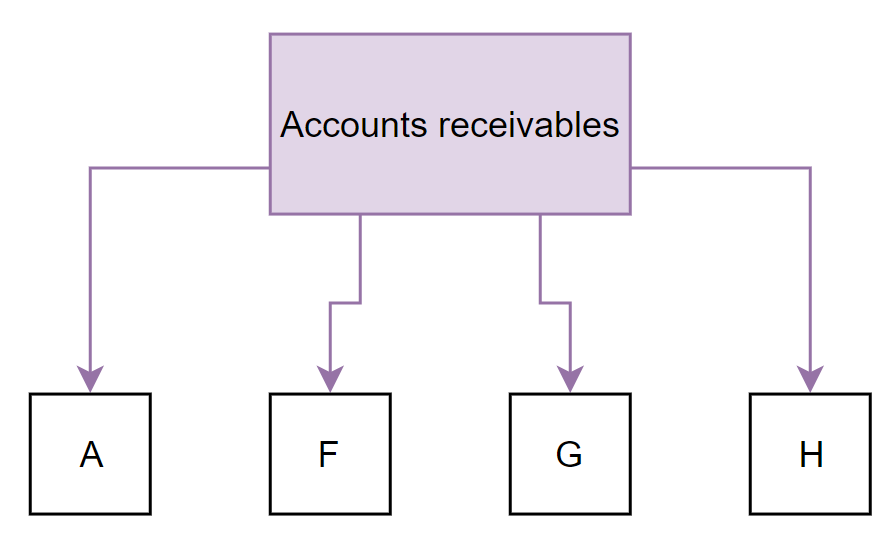
\includegraphics[width=5cm]{accountreceivables.png}
	\caption{Accounts receivables communiceert met volgende microservices.}
	\centering
\end{figure}
Accounts receivable gaat na of de betaling wel goed wordt afgerond. Hiervoor worden volgende microservices aangesproken:
\begin{itemize}
	\item Klantengegevens ophalen.
	\item Facturen maken en ophalen.
	\item Bericht plaatsen op queue.
	\item Bericht van queue halen.
\end{itemize}

\subsubsection{Klant management}
\begin{figure}[h!]
	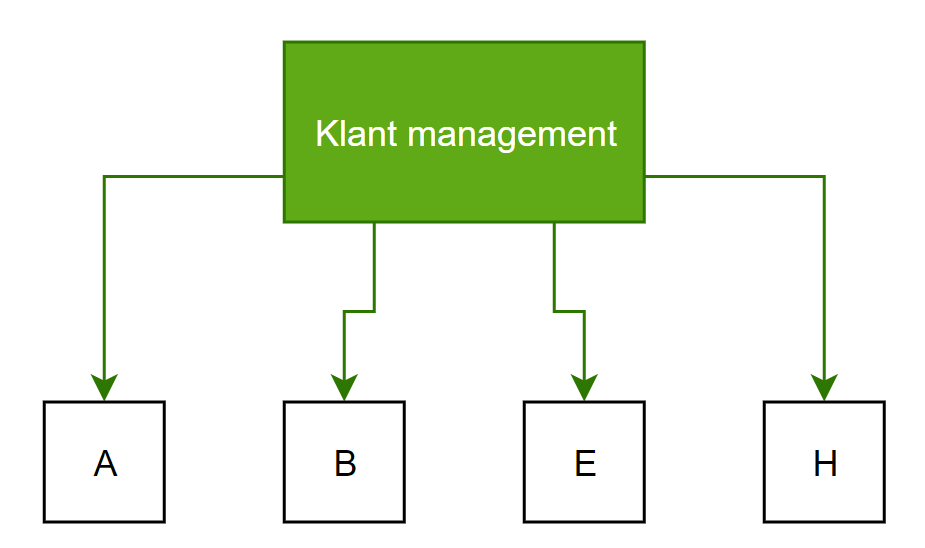
\includegraphics[width=5cm]{klantmanagement.png}
	\caption{Klant management communiceert met volgende microservices.}
	\centering
\end{figure}
Klant management staat in voor het contact met de klant. Dit onderdeel gebruikt volgende microservices:
\begin{itemize}
	\item Klanentgegevens ophalen.
	\item Orders ophalen, plaatsen en verwijderen.
	\item Facturen maken en ophalen.
	\item Bericht van queue halen.
\end{itemize}
Als een van de vorige onderdelen een bericht plaatst op deze queue, zal het bericht verwerkt worden. Daarna wordt de klant verwittigd met de inhoud van het bericht. Bijvoorbeeld als de klant geen order mag bestellen omdat Credit management nog onbetaalde facturen gevonden heeft, wordt de klant hiervan op de hoogte gebracht via klant management.


\section{De complete architectuur opbouwen}
Op figuur 3.11 is te zien hoe het proces in elkaar ziet. Door de microservice architectuur toe te passen op het order-to-cash proces verandert er niks aan de volgorde van het proces of het doel van het proces. De manier waarop gegevens worden opgehaald, verandert wel. 


\subsection{De volgende stappen: Het toevoegen van API, logging en authenticatie en authorisatie}
\subsubsection{Logging}
Logging kan toegepast worden door nog een extra microservice te ontwikkelen. Hiernaar kunnen de andere microservices dan hun logs naar posten. Dit wordt gebruikt om fouten in de architectuur te ontdekken. Hier zal echter niet verder op worden ingegaan. 

\subsubsection{API gateway}
Een API gateway wordt toegevoegd om ervoor te zorgen dat de architctuur niet openbaar is voor iedereen. Op die manier is er één aanspreekpunt en die regelt de rest van de communicatie.
De API communiceert in dit geval enkel met order management. Het geeft alle nodige informatie door en order management schrijft deze weg naar de databank.
\begin{figure}[h!]
	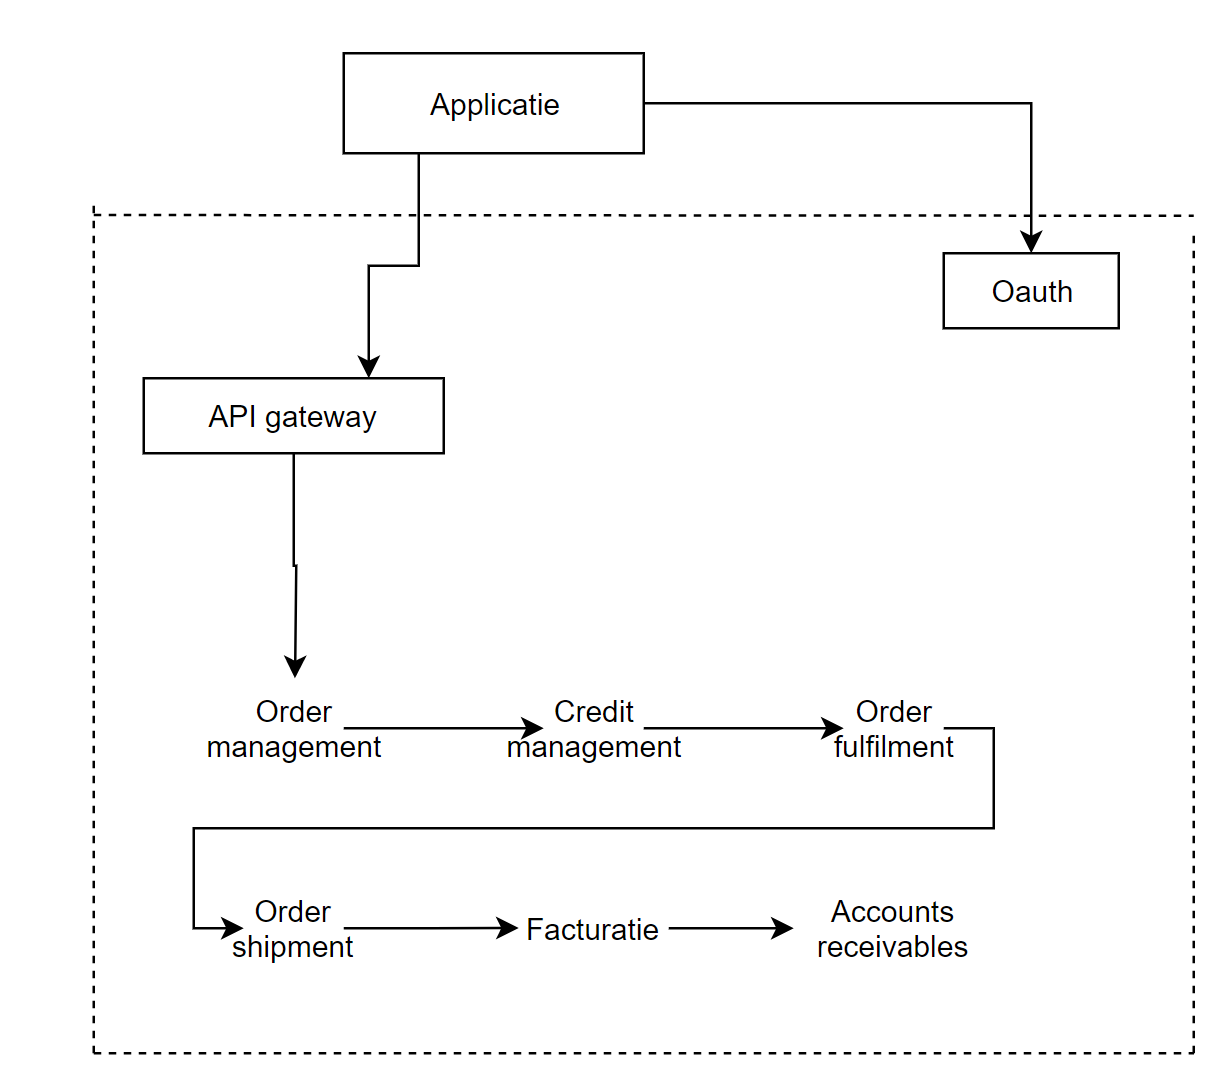
\includegraphics[width=10cm]{apiSchema.png}
	\caption{Vereenvoudigd schema.}
	\centering
\end{figure}

\subsubsection{Authenticatie en autorisatie}
Onder het hoofdstuk 'Stand Van Zaken', is er meer info te vinden over authenticatie. Uit die vergelijking, is API gekozen als authenticatie. Zoals we ook gezien hebben in het vorige hoofdstuk is API uit de verschillende opties gekozen, specifiek is er gekozen voor OAuth omdat dit de meest bekende en gebruikte versie is.

De gebruiker moet gekend zijn om een order te kunnen plaatsen. Er is een aparte micrservice voor authenticatie. Hier wordt niet dieper op in gegaan omdat het niet de essentie is van deze bachelorproef.





% Voeg hier je eigen hoofdstukken toe die de ``corpus'' van je bachelorproef
% vormen. De structuur en titels hangen af van je eigen onderzoek. Je kan bv.
% elke fase in je onderzoek in een apart hoofdstuk bespreken.

%\input{...}
%\input{...}
%...

%%=============================================================================
%% Conclusie
%%=============================================================================

\chapter{Conclusie}
\label{ch:conclusie}

% TODO: Trek een duidelijke conclusie, in de vorm van een antwoord op de
% onderzoeksvra(a)g(en). Wat was jouw bijdrage aan het onderzoeksdomein en
% hoe biedt dit meerwaarde aan het vakgebied/doelgroep? 
% Reflecteer kritisch over het resultaat. In Engelse teksten wordt deze sectie
% ``Discussion'' genoemd. Had je deze uitkomst verwacht? Zijn er zaken die nog
% niet duidelijk zijn?
% Heeft het onderzoek geleid tot nieuwe vragen die uitnodigen tot verder 
%onderzoek?

De conclusie van deze theoretische studie zal in dit deel duidelijk worden.

Als eerste werd de vraag 'Wat zijn microservices?' gesteld. 
Microservices zijn kleine delen die elk een requirement omvatten. Elke microservice functioneert apart en heeft weinig tot geen communicatie met de andere microservices. Om microservices te gaan ontwikkelen, moet er veel onderzocht worden. Wat te merken is aan de literatuurstudie. De literatuurstudie is niet heel diepgaand maar probeert wel zo veel mogelijk aspecten van microservices aan te halen. Microservice kan in meerdere contexten voor komen. Binnen elke context zal er meer verkaring nodig zijn. 

De volgende vraag was 'Hoe kan er overgeschakeld worden naar een microservice architectuur?'.
Er kan op verschillende manieren overgeschakeld worden naar microservices. Maar de meest aangeraden manier is: systematisch requirements vaststellen en omzetten naar een microservices. In een stappenplan werken, zodat er geen chaos ontstaat bij de overschakeling. Eerst de kern opbouwen en dan alle andere zaken erbij brengen. Eens de kern van de architectuur is getekend, kan men authenticatie, authorisatie, bescherming, logging en de API gateway er in steken. Er moet eerst goed worden nagedacht over hoe de implementatie van authenticatie, authorisatie, bescherming en logging zal gebeuren. Voor de overschakeling kan er gekeken worden naar de manier waarop men nu de authenticatie, authorisatie, bescherming en logging toepast en die manier dan verwerken bij de microservices.  

Daarna kwam 'Welke aanpassingen kunnen of moeten er gebeuren aan de architectuur om microservices te laten werken? De veranderingen worden hieronder opgesomd:
\begin{itemize}
	\item Heeft deze applicatie nood aan een microservice architectuur?
	\item De databank structuur moet herbekeken worden.
	\item Het volledige proces herbekijken.
	\item De manier van communiceren tussen de verschillende onderdelen moet worden onderzocht.
	\item Welke manier van authenticatie en authorisatie gaat men gebruiken?
	\item Welke manier van bescherming kan er toegepast worden?
	\item Moeten we de teams herstructureren?
\end{itemize}

Een andere vraag die in het begin gesteld werd: Hoe zal de communicatie tussen de verschillende microservices werken?
Voor de communicatie zijn er veel verschillende opties. Er moet gekeken worden naar welke manier het beste bij het bedrijf past. Is er een manier die al gekend is in het bedrijf? Heeft een andere manier enkele voordelen ten opzichte van de huidige techniek. In deze studie is er gekozen voor volgend communicatie methode: Via message queues. De data die microservice B nodig heeft, zal door microservice A naar microservice B zijn queue worden gestuurd. Bij deze manier heeft elke microservice een queue. Heeft microservice A data doorgekregen en haar taak ermee gedaan, dan plaatst ze een link naar de data op de queue van de microservice die de data nodig heeft. Dit zorgt ervoor dat als microservice B uitvalt, de nodige data niet verloren gaat. De queue slaat de gegevens op en verwijdert ze pas als ze zijn opgehaald. Als deze methode niet past binnen de verwachtingen van de architectuur dan kan men onderzoeken welke methode beter is. 

Als volgt werd deze vraag gesteld: Hoe ziet een order-to-cash proces eruit? 
Het order-to-cash proces is een proces dat voorkomt bij het plaatsen van een order tot het betalen van de factuur. In volgende opsomming zijn de stappen terug te vinden:
\begin{enumerate}
	\item Order management
	\item Credit management
	\item Order fulfilment
	\item Order shipping
	\item Facturatie
	\item Accounts receivables
\end{enumerate}

De voorlaatste vraag, klinkt als volgt: Welke business requirements heeft een order-to-cash proces?
De belangrijkste requirement is dat de klant zijn bestelling krijgt. Een andere requirement is de wanbetalers minimaal te houden door ze vroeg in het proces er uit te halen. De requirements liggen in lijn met de noden van de klant. De business requirements werden opgesteld door het order-to-cash proces grondig te bestuderen. In de literatuurstudie is meer uitleg te vinden over het OTC proces.

Als laatste vraag werd 'Welke invloed heeft de microservice architectuur op de performance van een order-to-cash proces?' gesteld.
Het verschil op performance vlak kan pas getest worden bij een studie met een proof of concept. Wat wel geconcludeerd kan worden, is volgende: De performance zal stabieler zijn bij pieken van orders. Omdat de microservices onafhankelijk zijn van elkaar. De onderdelen van het OTC proces kunnen onafhankelijker functioneren. Valt er een onderdeel uit of tijdelijk niet beschikbaar dan heeft dat geen grote gevolgen voor het proces in het algemeen. Het onderdeel ervoor kan nog altijd data op de queue plaatsen. Maar de onderdelen na het onbeschikbare deel, zal wel wat hinder ondervinden. Maar niet zodat het gehele proces plat zal liggen.


Microservice is een architectuur en ideologie waarin logica en de requirements, die te vinden zijn bij een monolithic, terugkomen. Dit heeft invloed op de overschakeling naar microservices. Deze manier van implementatie moet aangepast worden bij het gebruik van microservices. Dat kan een obstakel zijn. Er wordt een andere manier van denken en organiseren gevraagd binnen een de IT-afdeling. De teams worden hervormd. Een team bevat niet meer de kennis van de volledige architectuur., enkel over de microservice waaraan zij werken. 


Ten slotte kan er geconcludeerd worden dat:
\begin{itemize}
	\item Microservices een brede term is en kan voorkomen in verschillende contexten.
	\item Een microservice architectuur niet altijd nodig is.
	\item Microservices kunnen een OTC proces automatiseren.
	\item Microservices zorgen ervoor dat elk onderdeel van het proces apart kan functioneren.
\end{itemize}

Zelf heb ik ondervonden dat het aanpassen van een monolithic niet eenvoudig is. De monolithic architectuur zit ingebakken in het informatica landschap. De manier van omgang met microservices, kan vergeleken worden met die van Agile. De Agile methode moest in eerste instatie zijn toegevoegde waarde op een project bewijzen. Dan pas zijn projectmanagers deze ook gaan gebruiken. Microservices zal eerst zijn voordeel moeten bewijzen ten opzichte van monolithic om een statement te kunnen maken.





%%=============================================================================
%% Bijlagen
%%=============================================================================

\appendix
\renewcommand{\chaptername}{Appendix}

%%---------- Onderzoeksvoorstel -----------------------------------------------

\chapter{Onderzoeksvoorstel}

Het onderwerp van deze bachelorproef is gebaseerd op een onderzoeksvoorstel dat vooraf werd beoordeeld door de promotor. Dat voorstel is opgenomen in deze bijlage.

% Verwijzing naar het bestand met de inhoud van het onderzoeksvoorstel
%---------- Inleiding ---------------------------------------------------------

\section{Introductie} % The \section*{} command stops section numbering
\label{sec:introductie}

Hoe Microservice integration patterns een order to cash proces in SAP beinvloedt. Dit onderwerp werd gekozen omdat deze nieuwe technology een interessante invloed kan hebben op de order-to-cash proces. Dit is een manier om een proces robuuster te maken. In de meeste software wordt gebruik gemaakt van één grote databank of meerdere databanken die in staan zijn om meerde services te voorzien van data. Bij microservice integration patterns wordt voor elke service een aparte databank opgesteld. Dit is maar een klein deeltje van een microservice. De microservices moeten voldoen aan business requirements. SAP zelf heeft ook al veel ondernomen omtrend microservices. Eén van hun oplossingen is Kyma. Maar de belangrijkste vraag is namelijk: Hoe microservice integration patterns een order-to-cash in SAP beïnvloedt. Deze bachelorproef zal voor het grootste deel een theoretische vergelijking zijn. Omdat deze studie als bachelorproef dient, is er maar beperkte tijd en resources om een onderzoek te doen. 

%---------- Stand van zaken ---------------------------------------------------

\section{Literatuurstudie}
\label{sec:state-of-the-art}

Over het onderwerp "Microservice Integration Patterns on Order-to-Cash proces in SAP", zijn er nauwelijks thesissen te vinden. De meeste informatie komt uit artikels die meer uitleg geven over microservices en artikels met een uitgebreide beschrijving over wat order-to-cash inhoudt.
Voor wie denkt dat microservices iets nieuws is, zit er een beetje naast. Grote bedrijven zoals Netflix, Twitter, Amazon en facebook maken al gebruik van deze technologie. ~\cite{CiderBlog2018}

\subsection{Wat zijn microservices?}
Het bouwen van aparte functies/modules met hun eigen interface en methoden. Deze manier van werken is in het voordeel van Agile. Bij Agile wordt er gewerkt met deeltjes software opleveren en opgeleverde software, daar wordt er zo goed als niks meer aan veranderd. Microservices worden onderverdeeld aan de hand van business requirements. Deels zorgen microservices ervoor dat er beter moet worden samengewerkt met de business.

\subsection{Waarom microservices gebruiken} 
In het artikel van ~\cite{Gunaratne2018} werd besproken hoe je een microservice werkt. En waarom deze gebruikt worden. Volgens dit artikel zijn microservices een goede, nieuwe techniek die op lange termijn huidige SOA's kan vervangen. 

~\cite{Atrash2018} beschrijft waarom je deze techniek kunt gebruiken, in de plaats van de kleinere SOA-services. Ook hier wordt verwezen naar de belangrijkheid van de requirements van de business. Door de grootte van deze services, is er de mogelijkheid om te caching. 

~\cite{devoteam2018} legt uit waarom microservices een kleine-SOA is. Een microservice omvat bepaalde, aanvullende, concepten omliggend deze 'kleinere services' en dit is waar ze beginnen met aantonen van de verschillen.

Is de integratie van microservices wel mogelijk? Deze vraag beantwoordt door ~\cite{VanBart2018}. Software wordt meestal nog geimplementeerd in de 3-tiers manier. Ook wel monolithic genoemd. De applicatie is uit een alleenstaande unit gemaakt. Eén verandering heeft een impact op de volledige applicatie. Is dit dan een geldige reden om voor microservices te kiezen? Dat hangt af van wat je applicatie percies nodig heeft. Niet alle applicaties worden er beter van om een microservice te implementeren. Een microservice  bestaat er uit om op zichzelf te werken. Dit wordt uitgelegd in het volgende deel.

\subsection{Principes voor Microservices Integration}

De principes van microservices integration werden uitgelegd in volgend artikel ~\cite{Aradheye2018}
In het artikel wordt op een duidelijke manier uitgelegd hoe microservices worden gebruikt. Microservices worden het best opgesteld aan de hand van business units. Een microservice wordt benaderd vanuit de business requirements. Deze hebben, volgens dit artikel, een betere performantie dan de huidig gebruikte techniek. Microservices worden opgedeeld in verschillende klasses. Bijvoorbeeld:
\begin{itemize}
	\item één voor klantendata
	\item één voor bestellingen
	\item één voor "wil-ik" lijsten
\end{itemize}

De belangrijkste eigenschappen van microservices zijn:
\begin{itemize}
	\item Microservice bestaat uit meerdere componenten
	\item Gemaakt voor de business
	\item Microservice maakt gebruik van simpele routing
	\item Een microservice is gedecentraliseerd
	\item Een microservice werkt zelfstandig
\end{itemize}

\subsection{Order-to-cash in SAP}
Order-to-cash is een van de vele processen in SAP die vast gelegd zijn. Dit proces legt uit hoe men van een bestelling naar de inning van het geld gaat. Er zijn verschillende versies van hoe het proces gaat. Volgens ~\cite{Akthar2018} verloopt het proces als volgt: er wordt een order geplaatst dan wordt die bestelling geleverd, daarna wordt er een factuur opgesteld en als laatste wordt het geld geind. Het proces op zich is niet ingewikkeld. ~\cite{OpenSap2018} geeft veel meer uitleg over wat er achter de schermen gebeurd. Bij dit proces wordt de financiële kant van SAP aangesproken, ook de verkoop en distributie alsook de stock worden aangesproken. Een gedetailleerder proces houdt in dat er een sales order gemaakt wordt. Dan wordt de stock bekeken. Afhankelijk van de beschikbaarheid van de goederen kan er een levering gepland worden. Zijn de goederen beschikbaar, dan kan er na de planning van de levering, effectief geleverd worden. Als volgt wordt er een factuur opgemaakt. Als laatste komt dan het betalingsproces. 

\subsection{Kyma}
Kyma is een open-source project van SAP. Het is vooral gebaseerd op Kubernetes. Op deze manier kan je oplossingen in de Cloud maken. Kyma is special omdat zij zo goed als alle oplossingen op één plek hebben. Zij hebben een application connector. Kyma is serverless. Ze maken service management eenvoudiger. ~\cite{Kyma2019}
Volgens het artikel van ~\cite{Semerdzhiev2018} is er meer nood aan openheid en een modernere architectuur. Dat is ook de reden waarom Kyma een open source project is. Kyma ondersteund container-based werken (zoals docker) alsook cloud-native apps. 

% Voor literatuurverwijzingen zijn er twee belangrijke commando's:
% \autocite{KEY} => (Auteur, jaartal) Gebruik dit als de naam van de auteur
%   geen onderdeel is van de zin.
% \textcite{KEY} => Auteur (jaartal)  Gebruik dit als de auteursnaam wel een
%   functie heeft in de zin (bv. ``Uit onderzoek door Doll & Hill (1954) bleek
%   ...'')

%---------- Methodologie ------------------------------------------------------
\section{Methodologie}
\label{sec:methodologie}
In dit werk gaan we onderzoeken op welke manier microservices een invloed zou kunnen hebben op een order-to-cash proces in SAP. De services die ze nu gebruiken vergelijken met microservices. Kunnen microservices de werking van SAP versnellen en performanter maken bij fouten? Welke messaging manier zou het beste kunnen zijn. 
Eerst willen we het volledige order-to-cash proces verstaan. Dan gaan we gaan onderzoeken welke verschillende mogelijkheden er zijn in verband met microservices. Kyma, PaaS.io of zijn er nog andere die een grote rol kunnen spelen. Ook moet er gekeken worden welke manier van communiceren tussen de microservices het beste is. Voor dit onderzoek zal er veel literatuur studie gedaan worden. 


%---------- Verwachte resultaten ----------------------------------------------
\section{Verwachte resultaten}
\label{sec:verwachte_resultaten}
Naar de gelezen literatuur kijkende, zou Kyma eigenlijk de beste oplossing moeten zijn. Deze is namelijk zelf afkomstig van SAP. Dit zou een goede oplossing moeten zijn. Maar zijn microservices wel haalbaar in een order-to-cash proces in SAP. Eerst zal dit duidelijk moeten worden vooraleer we gaan kijken naar welke microservice de best mogelijk noden opvult. 


%---------- Verwachte conclusies ----------------------------------------------
\section{Verwachte conclusies}
\label{sec:verwachte_conclusies}

De conclusie die we uit dit onderzoek  kunnen trekken: microservices integration patterns zijn voordeliger en gebruiksvriendelijker dan het huidige systeem is voor de mensen die de software gaan gebruiken. Bij fouten aan een service, zal het platform nog beschikbaar zijn. Het risico is wel dat door de relatief nieuwe techniek, er enkele dingen niet zullen lopen zoals we zouden willen. Het is mogelijk dat we maar tot een gedeeltelijke conclusie komen.



%%---------- Andere bijlagen --------------------------------------------------
% TODO: Voeg hier eventuele andere bijlagen toe
%\input{...}

%%---------- Referentielijst --------------------------------------------------

\printbibliography[heading=bibintoc]

\end{document}
